% Model-form versus finite-sampling uncertainty in micromagnet-assisted spin--valley shuttling: a periodic-reference sensitivity atlas
% Target journal: Journal of Applied Physics (AIP; REVTeX 4-2, jap substyle).
%
% Build:
%   pdflatex paper
%   bibtex paper
%   pdflatex paper
%   pdflatex paper

\documentclass[aip,jap,reprint,superscriptaddress,longbibliography,floatfix]{revtex4-2}
\pdfoutput=1
\usepackage[T1]{fontenc}
\usepackage{amsmath,amssymb,graphicx,bm}
\usepackage{booktabs}
\usepackage[scaled=0.92]{helvet}
\usepackage[eulergreek]{sansmath}
\usepackage{pifont} % sans fonts in Fig.~1 to match matplotlib figures

\usepackage{tikz}
\usetikzlibrary{arrows.meta,positioning,patterns,backgrounds,fit,calc}
\usepackage{xcolor}
\definecolor{bzblue}{RGB}{31,119,180}
\definecolor{bxorange}{RGB}{214,96,20}
\definecolor{robustteal}{RGB}{56,142,142}
\definecolor{deadgray}{RGB}{225,225,225}
\definecolor{panelgray}{RGB}{150,150,150}
% model colors matched to Fig. 2 (Tol vibrant palette)
\definecolor{tolA}{HTML}{0077bb}
\definecolor{tolAp}{HTML}{33bbee}
\definecolor{tolBz}{HTML}{009988}
\definecolor{tolBx}{HTML}{ee7733}

\usepackage[colorlinks=true,allcolors=blue]{hyperref}
\hypersetup{pdftitle={Model-form versus finite-sampling uncertainty in micromagnet-assisted spin-valley shuttling}, pdfauthor={Inuk You}}

\begin{document}

\title{Model-form versus finite-sampling uncertainty in
micromagnet-assisted spin--valley shuttling: a periodic-reference
sensitivity atlas}

\author{Inuk You}
\email{youinuk@gmail.com}
\affiliation{Department of Science, Kyungdong High School, Seoul, Republic of Korea}

\date{\today}

\begin{abstract}
Coherent spin shuttling in Si/SiGe couples spin dynamics to the valley degree of
freedom, but a design calculation must assume an effective local spin--valley
coupling profile, and that profile is not uniquely fixed for the moving-dot
micromagnet setting considered here. We quantify how strongly a design-facing
classification depends on that choice and compare the dependence with the
variation finite Monte-Carlo sampling produces on its own. Using a periodic
micromagnet array as a controlled-reference geometry, we evaluate 108
conditions under four phenomenological coupling ans\"atze. Within each seed
block all four share the same noise realizations; independent seed blocks
supply a same-ansatz sampling benchmark. At the pre-registered endpoint of 30
realizations the two disagreement rates are nearly equal, 0.388 and 0.385. In a
registered follow-up to 100 realizations, cross-ansatz disagreement stays at
0.395 while cross-seed disagreement falls to 0.298. The balance is response
dependent: at 100 realizations cross-ansatz disagreement is comparable to the
sampling benchmark for valley excitation but 5.60 times as large for spin
dephasing. A post-hoc diagnostic shows that similar rankings of response
magnitude need not imply similar thresholded classifications, and operating
points selected for stability across noise samples transport unevenly across
the four profiles. Design conclusions drawn under a single phenomenological
coupling profile therefore remain model-conditional unless the coupling is
independently constrained or robustness is demonstrated across a justified
model family.
\end{abstract}

\maketitle

\section{Introduction}


\begin{figure*}[p]
\centering
% ================= Figure 1 (overview) =================
% Layout: (a) pseudo-3D device with aligned \varepsilon_v / gradient profiles
%         (b) four coupling ansaetze (2x2 minis)
%         (c) experiment block diagram with the two registered endpoints
%         (d) matched comparison: (d1) n trajectory, (d2) pairwise spread
%         bottom: one-line message bar
% ================= Figure 1 (overview, full-page) =================
% (a) pseudo-3D device (rectangular Co micromagnet bars, xyz triad,
%     150nm period scale bar, tilted spin arrow through the qubit)
%     + x-aligned \varepsilon_v / gradient profiles
% (b) four coupling ansaetze, 4 stacked rows sharing the x axis
%     (pocket band and \varepsilon_v=E_Z hot-spot guides labelled)
% (c) vertical experiment flowchart ending in the two registered endpoints
% (d) (d1) D_ansatz / D_seed against n_real, eight registered checkpoints;
%     (d2) the six ansatz pairs and ten seed pairs at n=100 on the same
%     vertical scale. Coordinates generated from attribution_n100.json.
% All text sans-serif (\sffamily + sansmath) to match Figs. 2-4.
{\sffamily\sansmath
\providecommand{\figDelta}{\varDelta}%
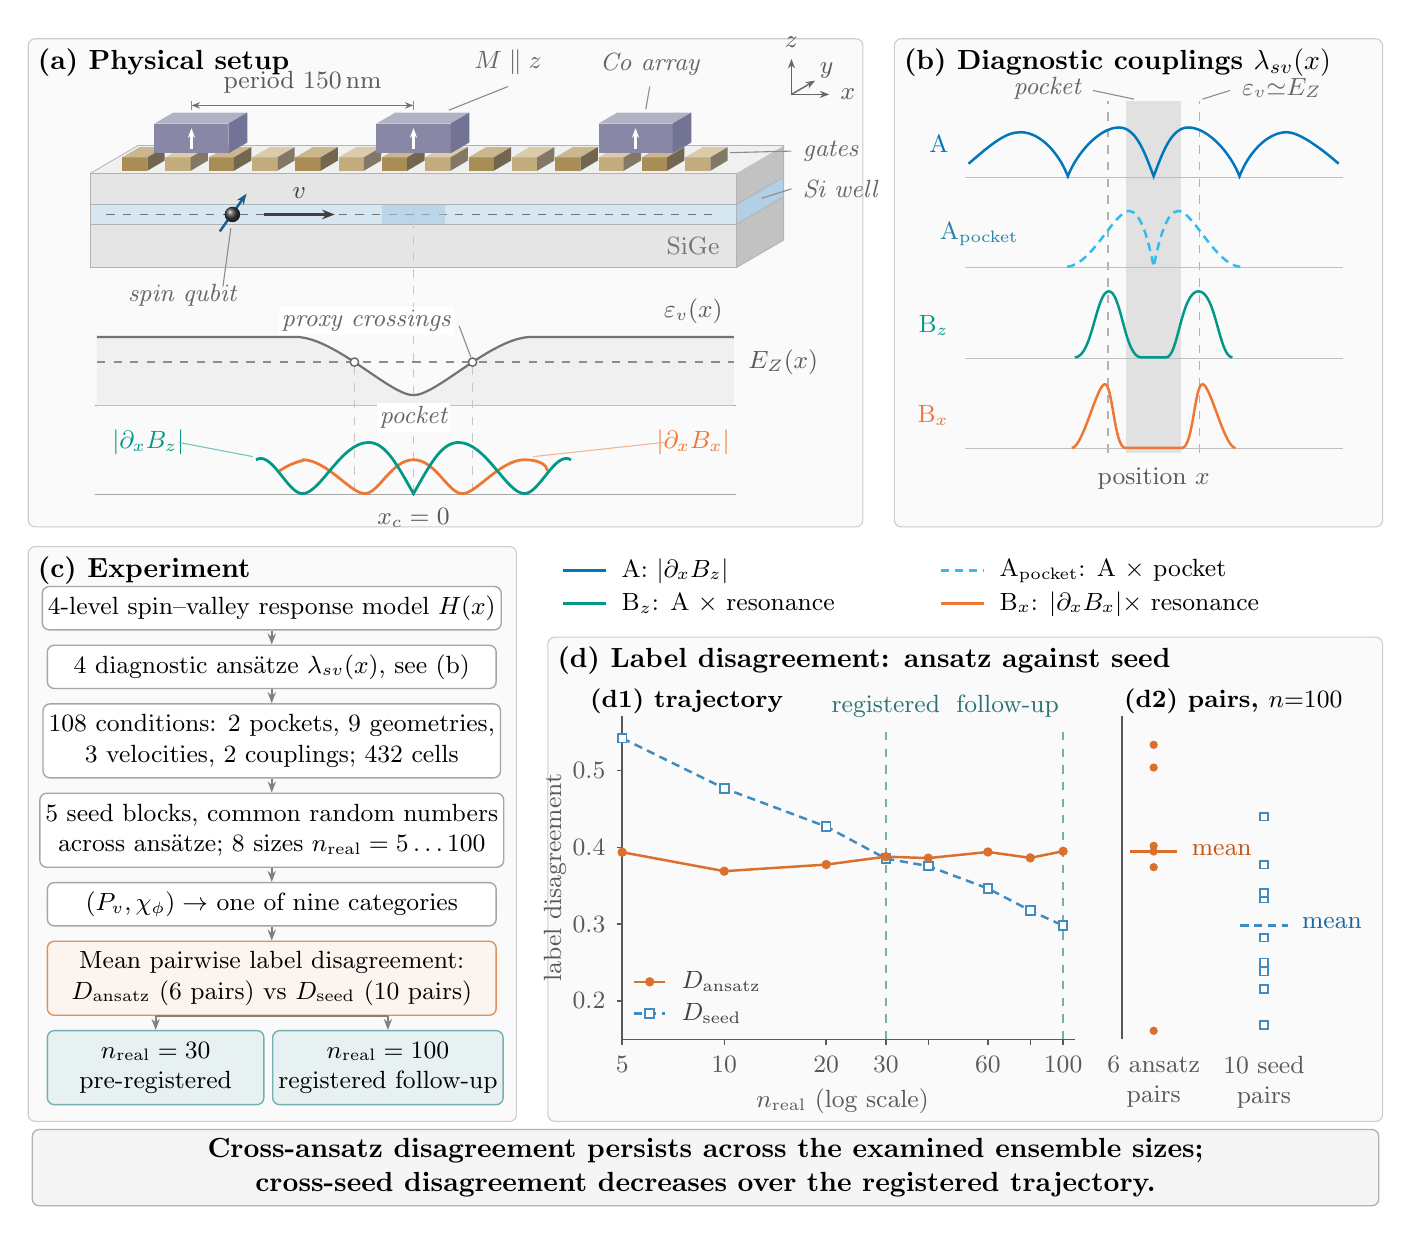
\begin{tikzpicture}[
  font=\normalsize,
  panel/.style={fill=black!2, draw=black!20, rounded corners=2.5pt, line width=0.4pt},
  ptitle/.style={anchor=north west, font=\normalsize\bfseries, inner sep=3.5pt},
  taglabel/.style={font=\small\itshape, text=black!60},
  leader/.style={black!45, line width=0.4pt},
  axisline/.style={black!65, line width=0.5pt},
  tick/.style={font=\small, text=black!65},
  pnode/.style={draw=black!35, fill=white, rounded corners=2.5pt, line width=0.5pt,
                align=center, font=\small, inner sep=2pt, minimum width=3.95cm,
                minimum height=0.55cm},
  pnode2/.style={pnode, minimum height=0.94cm},
  parrow/.style={-{Stealth[length=1.4mm]}, line width=0.7pt, black!50},
]
\colorlet{gategold}{yellow!35!orange!55!black!85}
\colorlet{gategoldlt}{gategold!70}
\colorlet{magsteel}{blue!25!black!55}

% =============================================================
%  (a) Physical setup
% =============================================================
\begin{scope}[shift={(0,0)}]
  \node[panel, minimum width=10.6cm, minimum height=6.2cm, anchor=south west] (pa) at (0,0) {};
  \node[ptitle] at (pa.north west) {(a) Physical setup};

  % ----- heterostructure stack (oblique dx=0.6, dz=0.35) -----
  \fill[black!10]  (0.8,3.30) rectangle (9.0,3.85);   % SiGe buffer
  \fill[black!24]  (9.0,3.30) -- (9.0,3.85) -- (9.6,4.20) -- (9.6,3.65) -- cycle;
  \fill[bzblue!18] (0.8,3.85) rectangle (9.0,4.10);   % Si quantum well
  \fill[bzblue!35] (9.0,3.85) -- (9.0,4.10) -- (9.6,4.45) -- (9.6,4.20) -- cycle;
  \fill[black!10]  (0.8,4.10) rectangle (9.0,4.50);   % SiGe barrier
  \fill[black!24]  (9.0,4.10) -- (9.0,4.50) -- (9.6,4.85) -- (9.6,4.45) -- cycle;
  \fill[black!6]   (0.8,4.50) -- (9.0,4.50) -- (9.6,4.85) -- (1.4,4.85) -- cycle;
  \draw[black!30, line width=0.3pt] (0.8,3.30) rectangle (9.0,4.50);
  \draw[black!30, line width=0.3pt] (0.8,3.85) -- (9.0,3.85) (0.8,4.10) -- (9.0,4.10);
  \draw[black!30, line width=0.3pt] (0.8,4.50) -- (1.4,4.85) -- (9.6,4.85) -- (9.6,3.65) -- (9.0,3.30);
  \draw[black!30, line width=0.3pt] (9.6,4.20) -- (9.0,3.85) (9.6,4.45) -- (9.0,4.10);
  \node[tick, text=black!55] at (8.45,3.57) {SiGe};

  % ----- shuttling gates (14 fingers on the surface) -----
  \foreach \gx [count=\i] in {1.15,1.70,2.25,2.80,3.35,3.90,4.45,5.00,5.55,6.10,6.65,7.20,7.75,8.30} {
    \ifodd\i \def\gcol{gategold}\else \def\gcol{gategoldlt}\fi
    \fill[fill=\gcol]        (\gx+0.05,4.53) rectangle (\gx+0.37,4.70);
    \fill[fill=\gcol!60]     (\gx+0.05,4.70) -- (\gx+0.37,4.70) -- (\gx+0.59,4.83) -- (\gx+0.27,4.83) -- cycle;
    \fill[fill=\gcol!60!black](\gx+0.37,4.53) -- (\gx+0.37,4.70) -- (\gx+0.59,4.83) -- (\gx+0.59,4.66) -- cycle;
  }

  % ----- micromagnet bars -----
  % Placed on the same horizontal scale as the profiles below: 150 nm =
  % 2.82 units, full width 50 nm = 0.94, and a bar centred on the profile
  % origin 4.90, which is a prism centre in the released array.
  % All prisms carry the SAME +z magnetization (periodic_array.py uses one
  % Ms for every prism); the arrows must not alternate.
  \foreach \mc in {2.08,4.90,7.72} {
    \fill[magsteel!85] (\mc-0.47,4.75) rectangle (\mc+0.47,5.13);
    \fill[magsteel!55] (\mc-0.47,5.13) -- (\mc+0.47,5.13) -- (\mc+0.71,5.27) -- (\mc-0.23,5.27) -- cycle;
    \fill[magsteel]    (\mc+0.47,4.75) -- (\mc+0.47,5.13) -- (\mc+0.71,5.27) -- (\mc+0.71,4.89) -- cycle;
    \draw[-{Stealth[length=1.2mm]}, white, line width=0.9pt] (\mc,4.81) -- (\mc,5.07);
  }

  % ----- period scale bar between magnet centres -----
  % Bar, ticks and label move down together; the magnet top faces reach 5.27,
  % so 5.30 is the lowest the tick feet can go.
  \draw[black!55, line width=0.5pt, {Stealth[length=1.1mm]}-{Stealth[length=1.1mm]}]
    (2.08,5.36) -- (4.90,5.36);
  \draw[black!45, line width=0.4pt] (2.08,5.30) -- (2.08,5.42) (4.90,5.30) -- (4.90,5.42);
  \node[tick, anchor=south] at (3.49,5.39) {period $150$\,nm};

  % ----- labels above -----
  \node[taglabel, anchor=south] at (6.1,5.62) {$M\parallel z$};
  \draw[leader] (6.1,5.60) -- (5.35,5.30);
  \node[taglabel, anchor=south] at (7.9,5.62) {Co array};
  \draw[leader] (7.9,5.60) -- (7.85,5.31);

  % ----- coordinate triad (top right) -----
  \draw[-{Stealth[length=1.2mm]}, black!60, line width=0.5pt] (9.7,5.50) -- (10.18,5.50);
  \draw[-{Stealth[length=1.2mm]}, black!60, line width=0.5pt] (9.7,5.50) -- (9.7,5.95);
  \draw[-{Stealth[length=1.2mm]}, black!60, line width=0.5pt] (9.7,5.50) -- (10.00,5.675);
  \node[tick, anchor=west] at (10.20,5.50) {$x$};
  \node[tick, anchor=south] at (9.7,5.97) {$z$};
  \node[tick, anchor=south west, inner sep=1pt] at (10.02,5.66) {$y$};

  % ----- moving spin qubit in the well -----
  \draw[black!55, dashed, line width=0.5pt] (1.0,3.975) -- (8.8,3.975);
  \draw[-{Stealth[length=1.6mm]}, black!75, line width=0.8pt] (3.0,3.975) -- (3.9,3.975);
  \node[tick, anchor=south, text=black!75] at (3.45,4.05) {$v$};
  \draw[-{Stealth[length=1.4mm]}, bzblue!80!black, line width=0.9pt] (2.44,3.76) -- (2.78,4.24);
  \shade[ball color=black!75] (2.6,3.975) circle (2.8pt);

  % pocket region marked in the well
  \fill[bzblue!40, opacity=0.55] (4.5,3.85) rectangle (5.3,4.10);

  % ----- side labels with leaders (routed clear of gates/magnets) -----
  \node[taglabel, anchor=west] at (9.72,4.78) {gates};
  \draw[leader] (9.70,4.78) -- (8.92,4.76);
  \node[taglabel, anchor=west] at (9.72,4.30) {Si well};
  \draw[leader] (9.70,4.30) -- (9.32,4.18);
  \node[taglabel, anchor=west] at (1.15,2.95) {spin qubit};
  \draw[leader] (2.48,3.06) -- (2.58,3.80);

  % ----- aligned profiles below -----
  % pocket-centre reference: well -> \varepsilon_v panel -> gradient panel
  \draw[black!22, dashed, line width=0.4pt] (4.9,4.12) -- (4.9,0.42);
  % centred-pocket placement: x_c sits on the array-symmetry point
  \node[tick, anchor=north] at (4.9,0.36) {$x_c=0$};
  % \varepsilon_v(x)
  \draw[axisline, black!35] (0.85,1.55) -- (9.0,1.55);
  \begin{scope}
    \clip (0.85,1.55) rectangle (9.0,2.55);
    \fill[deadgray!50]
      (0.88,2.42) -- (3.40,2.42)
      .. controls (3.90,2.42) and (4.60,1.68) .. (4.90,1.68)
      .. controls (5.20,1.68) and (5.90,2.42) .. (6.40,2.42)
      -- (8.97,2.42)
      -- (8.97,1.55) -- (0.88,1.55) -- cycle;
  \end{scope}
  \draw[black!55, line width=0.8pt]
    (0.88,2.42) -- (3.40,2.42)
    .. controls (3.90,2.42) and (4.60,1.68) .. (4.90,1.68)
    .. controls (5.20,1.68) and (5.90,2.42) .. (6.40,2.42)
    -- (8.97,2.42);
  \draw[black!45, dashed, line width=0.5pt] (0.88,2.10) -- (8.97,2.10);
  \node[tick, anchor=west, align=left] at (9.03,2.10)
        {$E_Z(x)$};
  \node[font=\small, text=black!65, anchor=south east] at (8.95,2.46) {$\varepsilon_v(x)$};
  \node[taglabel, fill=white, inner sep=1.2pt] at (4.9,1.40) {pocket};
  \draw[black!60, fill=white, line width=0.5pt] (4.15,2.10) circle (1.5pt);
  \draw[black!60, fill=white, line width=0.5pt] (5.65,2.10) circle (1.5pt);
  \node[taglabel, anchor=east, fill=white, inner sep=1.2pt]
        at (5.42,2.62) {proxy crossings};
  \draw[leader] (5.48,2.56) -- (5.63,2.16);
  % guides from hot spots to the gradient lobes
  \draw[black!22, dashed, line width=0.4pt] (4.15,2.04) -- (4.15,0.44);
  \draw[black!22, dashed, line width=0.4pt] (5.65,2.04) -- (5.65,0.44);
  % gradient components: symmetric about the pocket centre, approximately
  % shifted (|dBz/dx| has a node at the centre; |dBx/dx| is maximal there)
  \draw[axisline, black!35] (0.85,0.42) -- (9.0,0.42);
  % Both components are periodic with the array. Drawn |dBx/dx| first so
  % that the longitudinal component, which the A-type kernels use, sits on
  % top where they overlap.
  % |dBx/dx|: maximum at the array symmetry point, node just INBOARD of the
  % hot-spot guides (code: node at +-33 nm), maximal again at +-75 nm.
  \draw[tolBx, line width=1.0pt]
    (3.20,0.72) .. controls (3.40,0.86) and (3.60,0.86) .. (3.49,0.86)
    .. controls (3.80,0.86) and (4.10,0.43) .. (4.28,0.43)
    .. controls (4.46,0.43) and (4.62,0.86) .. (4.90,0.86)
    .. controls (5.18,0.86) and (5.34,0.43) .. (5.52,0.43)
    .. controls (5.70,0.43) and (6.00,0.86) .. (6.31,0.86)
    .. controls (6.50,0.86) and (6.60,0.79) .. (6.60,0.72);
  % |dBz/dx|: node at the array symmetry point (and at +-75 nm), maxima
  % INBOARD of the hot-spot guides (code: max at +-30.2 nm vs hot spots at
  % +-39.9 nm), so the hot spot sits on the falling flank.
  \draw[tolBz, line width=1.0pt]
    (2.90,0.86) .. controls (3.10,0.98) and (3.30,0.43) .. (3.49,0.43)
    .. controls (3.72,0.43) and (3.98,1.08) .. (4.33,1.08)
    .. controls (4.55,1.08) and (4.70,0.78) .. (4.90,0.43)
    .. controls (5.10,0.78) and (5.25,1.08) .. (5.47,1.08)
    .. controls (5.82,1.08) and (6.08,0.43) .. (6.31,0.43)
    .. controls (6.50,0.43) and (6.70,0.98) .. (6.90,0.86);
  % The two component labels sit on the empty flanks of the band rather than
  % on top of each other at the centre: |dBz/dx| is drawn over 2.90--6.90 and
  % |dBx/dx| over 3.20--6.60, so x<2.9 and x>6.9 are free at this height.
  % Leaders carry the association; no white fill, which would mask the curves.
  \node[tolBz, font=\small, anchor=west] at (0.95,1.08) {$|\partial_x B_z|$};
  \draw[tolBz!55, line width=0.4pt] (1.92,1.08) -- (2.86,0.90);
  \node[tolBx, font=\small, anchor=east, inner sep=0.8pt]
        at (8.95,1.08) {$|\partial_x B_x|$};
  \draw[tolBx!55, line width=0.4pt] (8.08,1.08) -- (6.42,0.90);

\end{scope}

% =============================================================
%  (b) Four coupling ansaetze (shared x axis, 4 stacked rows)
% =============================================================
\begin{scope}[shift={(11.0,0)}]
  \node[panel, minimum width=6.2cm, minimum height=6.2cm, anchor=south west] (pb) at (0,0) {};
  \node[ptitle] at (pb.north west) {(b) Diagnostic couplings $\lambda_{sv}(x)$};

  % shared pocket band + hot-spot guides across all four rows
  \fill[deadgray] (2.95,0.95) rectangle (3.65,5.42);
  \draw[black!30, dashed, line width=0.4pt] (2.72,0.95) -- (2.72,5.42);
  \draw[black!30, dashed, line width=0.4pt] (3.88,0.95) -- (3.88,5.42);
  \node[taglabel, anchor=east] at (2.50,5.58) {pocket};
  \draw[leader] (2.53,5.55) -- (3.05,5.44);
  \node[taglabel, anchor=west] at (4.30,5.58) {$\varepsilon_v{\simeq}E_Z$};
  \draw[leader] (4.27,5.55) -- (3.92,5.44);

  % rows: baselines 4.45 / 3.30 / 2.15 / 1.00
  \foreach \b in {4.45,3.30,2.15,1.00}
    \draw[black!25, line width=0.4pt] (0.9,\b) -- (5.7,\b);

  % A : |dBz/dx| itself -- arches with V-zeros at the centre and at
  % +- half period (rising again beyond), cf. Fig. 2; peaks inboard of
  % the proxy crossings
  \node[font=\small, anchor=east, text=tolA] at (0.82,4.87) {A};
  \draw[tolA, line width=0.9pt]
    (0.95,4.62) .. controls (1.25,4.88) and (1.42,5.02) .. (1.61,5.02)
    .. controls (1.86,5.02) and (2.10,4.75) .. (2.21,4.46)
    .. controls (2.32,4.75) and (2.61,5.08) .. (2.86,5.08)
    .. controls (3.08,5.08) and (3.19,4.75) .. (3.30,4.46)
    .. controls (3.41,4.75) and (3.52,5.08) .. (3.74,5.08)
    .. controls (3.99,5.08) and (4.28,4.75) .. (4.39,4.46)
    .. controls (4.50,4.75) and (4.74,5.02) .. (4.99,5.02)
    .. controls (5.12,5.02) and (5.35,4.88) .. (5.65,4.62);

  % A_pocket : gradient x pocket-Gaussian -> twin peaks meeting in a
  % V-touch at the centre (|dBz/dx| ~ |x| near the node), Gaussian decay
  % anchored west so the leading A lines up with the B_z / B_x labels below
  \node[font=\small, anchor=west, text=tolAp!70!black] at (0.46,3.72) {$\mathrm{A_{pocket}}$};
  % peaks at +-21.39 nm -> 2.99 / 3.61, inboard of A's +-30.22 nm because
  % the pocket Gaussian pulls them toward the centre.
  \draw[tolAp, line width=0.9pt, densely dashed]
    (2.20,3.31) .. controls (2.52,3.34) and (2.80,4.02) .. (2.99,4.02)
    .. controls (3.14,4.02) and (3.24,3.62) .. (3.30,3.31)
    .. controls (3.36,3.62) and (3.46,4.02) .. (3.61,4.02)
    .. controls (3.80,4.02) and (4.08,3.34) .. (4.40,3.31);

  % B_z : resonance window, symmetric twin peaks on both flanks
  \node[font=\small, anchor=east, text=tolBz] at (0.82,2.57) {$\mathrm{B}_z$};
  % peaks at +-39.37 nm -> 2.73 / 3.87, just inside the +-39.91 nm guides
  \draw[tolBz, line width=0.9pt]
    (2.30,2.16) .. controls (2.52,2.16) and (2.57,3.00) .. (2.73,3.00)
    .. controls (2.89,3.00) and (2.93,2.16) .. (3.14,2.16)
    -- (3.46,2.16)
    .. controls (3.61,2.16) and (3.65,3.00) .. (3.87,3.00)
    .. controls (4.09,3.00) and (4.13,2.16) .. (4.30,2.16);

  % B_x : resonance window, same flanks but narrower / phase-shifted
  \node[font=\small, anchor=east, text=tolBx] at (0.82,1.42) {$\mathrm{B}_x$};
  % Peaks at +-42.60 nm -> 2.68 / 3.92, just OUTBOARD of the +-39.91 nm
  % guides, where B_z peaks just inboard. All four curves in this panel
  % are placed at their computed peak positions on a common x scale.
  \draw[tolBx, line width=0.9pt]
    (2.26,1.01) .. controls (2.40,1.01) and (2.58,1.82) .. (2.68,1.82)
    .. controls (2.78,1.82) and (2.80,1.01) .. (2.94,1.01)
    -- (3.66,1.01)
    .. controls (3.80,1.01) and (3.82,1.82) .. (3.92,1.82)
    .. controls (4.02,1.82) and (4.20,1.01) .. (4.34,1.01);

  \node[tick] at (3.3,0.62) {position $x$};
\end{scope}

% =============================================================
%  (c) Analysis pipeline (vertical flowchart)
% =============================================================

% ---- global ansatz legend between the panel rows ----
% line 1: gradient-only family; line 2: resonance-window family.
% Line styles must match panel (b): A solid, A_pocket densely dashed,
% B_z solid, B_x solid.
% Placed in the band above panel (d), which is shorter than panel (c);
% panel (c) occupies x < 6.2 at these heights, so the legend starts at 6.8.
\begin{scope}[shift={(0,-0.55)}]
  \draw[tolA, line width=1.0pt] (6.80,0) -- (7.35,0);
  \node[font=\small, anchor=west] at (7.42,0)
    {A: $|\partial_x B_z|$};
  \draw[tolAp, line width=1.0pt, densely dashed] (11.60,0) -- (12.15,0);
  \node[font=\small, anchor=west] at (12.22,0)
    {$\mathrm{A_{pocket}}$: A $\times$ pocket};
\end{scope}
\begin{scope}[shift={(0,-0.97)}]
  \draw[tolBz, line width=1.0pt] (6.80,0) -- (7.35,0);
  \node[font=\small, anchor=west] at (7.42,0)
    {$\mathrm{B}_z$: A $\times$ resonance};
  \draw[tolBx, line width=1.0pt] (11.60,0) -- (12.15,0);
  \node[font=\small, anchor=west] at (12.22,0)
    {$\mathrm{B}_x$: $|\partial_x B_x| \times$ resonance};
\end{scope}

\begin{scope}[shift={(0,-7.55)}]
  \node[panel, minimum width=6.2cm, minimum height=7.30cm, anchor=south west] (pc) at (0,0) {};
  \node[ptitle] at (pc.north west) {(c) Experiment};

  % Vertical layout: uniform 0.195 cm edge-to-edge gaps. Box heights are pinned
  % by minimum height (0.55 cm for one line, 0.94 cm for two) rather than left
  % to the glyph extents, so the gap is the same everywhere by construction.
  % Stack: top edge 6.80, bottom edge 0.22, six gaps of 0.195.
  % Every line is measured to fit 5.7 cm minus 2 x 2 pt: the widest is
  % "5 seed blocks, common random numbers" at 151.2 pt against 157.8 pt.
  \node[pnode, minimum width=5.7cm] (n1) at (3.1,6.525)
    {4-level spin--valley response model $H(x)$};
  \node[pnode, minimum width=5.7cm] (n2) at (3.1,5.78)
    {4 diagnostic ans\"atze $\lambda_{sv}(x)$, see (b)};
  \node[pnode2, minimum width=5.7cm] (n3) at (3.1,4.84)
    {108 conditions: 2 pockets, 9 geometries,\\ 3 velocities, 2 couplings; 432 cells};
  \node[pnode2, minimum width=5.7cm] (n4) at (3.1,3.705)
    {5 seed blocks, common random numbers\\
     across ans\"atze; 8 sizes $n_{\mathrm{real}}=5\ldots100$};
  \node[pnode, minimum width=5.7cm] (n5) at (3.1,2.765)
    {$(\figDelta P_v,\figDelta\chi_\phi)\to$ one of nine categories};
  \node[pnode2, minimum width=5.7cm, draw=bxorange!70, fill=bxorange!7] (n6) at (3.1,1.825)
    {Mean pairwise label disagreement:\\
     $D_{\mathrm{ansatz}}$ (6 pairs) vs $D_{\mathrm{seed}}$ (10 pairs)};
  \node[pnode2, fill=robustteal!12, draw=robustteal!70, minimum width=2.75cm]
    (c1) at (1.625,0.69) {$n_{\mathrm{real}}=30$\\ pre-registered};
  \node[pnode2, fill=robustteal!12, draw=robustteal!70, minimum width=2.75cm]
    (c2) at (4.575,0.69) {$n_{\mathrm{real}}=100$\\ registered follow-up};

  \draw[parrow] (n1) -- (n2);
  \draw[parrow] (n2) -- (n3);
  \draw[parrow] (n3) -- (n4);
  \draw[parrow] (n4) -- (n5);
  \draw[parrow] (n5) -- (n6);
  % fork from the matched comparison to the two registered endpoints
  \draw[parrow] (n6.south -| c1) -- (c1.north);
  \draw[parrow] (n6.south -| c2) -- (c2.north);
  \draw[black!50, line width=0.7pt] (n6.south -| c1) -- (n6.south -| c2);
\end{scope}

% =============================================================
%  (d) Matched comparison: trajectory and pairwise spread
% =============================================================
% Coordinates generated from attribution_n100.json, 2026-08-15.
% d1 plot box x in [0.95,6.55], y in [1.05,5.05]; x is log10(n) from
% n=5 to n=100; y is label disagreement from 0.15 to 0.56.
% d2 shares the same y mapping, so the pair spread and the aggregate
% curves are read on one vertical scale.
\begin{scope}[shift={(6.6,-7.55)}]
  \node[panel, minimum width=10.6cm, minimum height=6.15cm, anchor=south west] (pd) at (0,0) {};
  \node[ptitle] at (pd.north west) {(d) Label disagreement: ansatz against seed};

  \node[font=\small\bfseries, anchor=north west] at (0.42,5.62)
    {(d1) trajectory};
  \node[font=\small\bfseries, anchor=north west] at (7.20,5.62)
    {(d2) pairs, $n{=}100$};

  % ---- axes ----
  \draw[axisline] (0.95,1.05) -- (0.95,5.15);
  \draw[axisline] (0.95,1.05) -- (6.70,1.05);
  \foreach \v/\y in {0.2/1.538, 0.3/2.513, 0.4/3.489, 0.5/4.465} {
    \draw[axisline] (0.88,\y) -- (0.95,\y);
    \node[tick, anchor=east] at (0.86,\y) {\v};
  }
  % all eight checkpoints get a tick; only six are labelled, because at
  % \small the labels for n=40 and n=80 collide on the log axis
  \foreach \x in {0.950, 2.246, 3.541, 4.299, 4.837, 5.595, 6.133, 6.550}
    \draw[axisline] (\x,1.05) -- (\x,0.98);
  \foreach \n/\x in {5/0.950, 10/2.246, 20/3.541, 30/4.299, 60/5.595, 100/6.550}
    \node[tick, anchor=north] at (\x,0.96) {\n};
  \node[tick, anchor=north] at (3.75,0.55) {$n_{\mathrm{real}}$ (log scale)};
  \node[tick, rotate=90, anchor=south] at (0.36,3.10) {label disagreement};

  % ---- registered endpoints ----
  \draw[robustteal!70, dashed, line width=0.5pt] (4.299,1.05) -- (4.299,5.01);
  \draw[robustteal!70, dashed, line width=0.5pt] (6.550,1.05) -- (6.550,5.01);
  \node[font=\small, text=robustteal!80!black, anchor=south, align=center]
    at (4.299,5.02) {registered};
  \node[font=\small, text=robustteal!80!black, anchor=south east, align=center]
    at (6.62,5.02) {follow-up};

  % ---- D_seed: open squares, dashed ----
  \draw[bzblue!85, densely dashed, line width=0.9pt]
    (0.950,4.874) -- (2.246,4.237) -- (3.541,3.751) -- (4.299,3.345)
    -- (4.837,3.250) -- (5.595,2.965) -- (6.133,2.685) -- (6.550,2.493);
  \foreach \x/\y in {0.950/4.874, 2.246/4.237, 3.541/3.751, 4.299/3.345,
                     4.837/3.250, 5.595/2.965, 6.133/2.685, 6.550/2.493}
    \draw[bzblue!85, fill=white, line width=0.7pt]
      (\x-0.055,\y-0.055) rectangle (\x+0.055,\y+0.055);

  % ---- D_ansatz: filled circles, solid ----
  \draw[bxorange!90, line width=0.9pt]
    (0.950,3.426) -- (2.246,3.185) -- (3.541,3.269) -- (4.299,3.369)
    -- (4.837,3.351) -- (5.595,3.429) -- (6.133,3.354) -- (6.550,3.438);
  \foreach \x/\y in {0.950/3.426, 2.246/3.185, 3.541/3.269, 4.299/3.369,
                     4.837/3.351, 5.595/3.429, 6.133/3.354, 6.550/3.438}
    \fill[bxorange!90] (\x,\y) circle (1.7pt);

  % ---- legend, placed in the empty lower-left of the plot box ----
  \draw[bxorange!90, line width=0.9pt] (1.10,1.78) -- (1.50,1.78);
  \fill[bxorange!90] (1.30,1.78) circle (1.7pt);
  \node[font=\small, text=black!75, anchor=west] at (1.58,1.78)
    {$D_{\mathrm{ansatz}}$};
  \draw[bzblue!85, densely dashed, line width=0.9pt] (1.10,1.38) -- (1.50,1.38);
  \draw[bzblue!85, fill=white, line width=0.7pt] (1.245,1.325) rectangle (1.355,1.435);
  \node[font=\small, text=black!75, anchor=west] at (1.58,1.38)
    {$D_{\mathrm{seed}}$};

  % ---- crossing annotation ----


  % =========== (d2) pairwise spread at n = 100 ===========
  \draw[axisline] (7.30,1.05) -- (7.30,5.15);
  \node[tick, anchor=north, align=center] at (7.70,0.96) {6 ansatz\\ pairs};
  \node[tick, anchor=north, align=center] at (9.10,0.96) {10 seed\\ pairs};

  % ansatz pairs -- all six distinct under the corrected convention
  \foreach \x/\y in {7.70/1.158, 7.70/3.236, 7.70/3.435, 7.70/3.507,
                     7.70/4.501, 7.70/4.790}
    \fill[bxorange!90] (\x,\y) circle (1.5pt);
  % seed pairs -- all ten given as centres, same form as above
  \foreach \y in {1.234, 1.686, 1.912, 2.025, 2.341,
                  2.839, 2.839, 2.906, 3.268, 3.878}
    \draw[bzblue!85, fill=white, line width=0.6pt]
      (9.10-0.05,\y-0.05) rectangle (9.10+0.05,\y+0.05);

  % means
  \draw[bxorange!90, line width=0.9pt] (7.40,3.438) -- (8.00,3.438);
  \draw[bzblue!85, line width=0.9pt, densely dashed] (8.80,2.493) -- (9.40,2.493);
  \node[font=\small, text=bxorange!90!black, anchor=west] at (8.06,3.447) {mean};
  \node[font=\small, text=bzblue!85!black, anchor=west] at (9.46,2.529) {mean};


\end{scope}

% =============================================================
%  BOTTOM: message bar
% =============================================================
\begin{scope}[shift={(0,-8.13)}]
  \node[draw=black!30, fill=black!4, rounded corners=2.5pt, line width=0.5pt,
        minimum width=17.1cm, minimum height=0.75cm, anchor=west,
        align=center, font=\normalsize] at (0.05,0)
    {\textbf{Cross-ansatz disagreement persists across the examined ensemble sizes;}\\
     \textbf{cross-seed disagreement decreases over the registered trajectory.}};
\end{scope}
\end{tikzpicture}}% end sffamily/sansmath group
\caption{\textbf{Overview.}
(a)~Device schematic: an electron spin (tilted arrow) is shuttled at constant
velocity $v$ through the Si quantum well of a Si/SiGe heterostructure, beneath a
periodic array of identical, uniformly $z$-magnetized rectangular Co prisms
(period 150\,nm; not to scale along $y$), a controlled-reference geometry
motivated by proposed shuttling-bus architectures. Below, aligned with the
device: the diabatic valley-detuning landscape $\varepsilon_v(x)$ of
Eq.~\eqref{eq:evx}, the input-detuning proxy crossings where
$\varepsilon_v(x)\simeq E_Z(x)=g\mu_B[B_{\rm ext}+B_z(x)]$ (circles), and the
gradient components $|\partial_x B_z|$ and $|\partial_x B_x|$, which are
approximately phase shifted in space. At the array-symmetry point $x=0$ the
former vanishes and the latter is maximal; the centred-pocket case places $x_c$
there, so the node--pocket coincidence follows from that placement and is not
forced (Sec.~\ref{sec:model}). $E_Z$ is drawn as a horizontal level for clarity;
the calculations use its full spatial dependence (Fig.~\ref{fig:profiles}).
(b)~The four coupling ans\"atze $\lambda_{sv}(x)$ on a common position axis; the
grey band marks the pocket and the dashed lines the proxy crossings. For a
centred pocket the resonance ans\"atze (B$_z$, B$_x$) activate symmetrically on
both flanks, with B$_x$ peaking slightly outboard of the $\partial_x B_z$-based
kernels on the same flanks. Curves are independently height-normalized; peak
positions are those of the released profiles. The two-line legend below the
upper row gives mnemonic descriptors for the four profiles; the kernels
themselves are defined in Sec.~\ref{sec:model}.
(c)~Experiment: 108 conditions, each evaluated under all four ans\"atze in each
of five seed blocks, with common random numbers shared across ans\"atze within a
block, at nested realization counts $n_{\rm real}=5\ldots100$. Each condition
receives a nine-category thresholded label. Cross-ansatz disagreement
$D_{\rm ansatz}$, averaged over the six ansatz pairs, is measured against
same-ansatz cross-seed disagreement $D_{\rm seed}$, averaged over the ten
seed-block pairs. $n_{\rm real}=30$ is the pre-registered endpoint;
$n_{\rm real}=100$ is the endpoint of a follow-up extension registered after the
$n_{\rm real}=30$ result was seen.
(d)~Disagreement is the mean fraction of conditions assigned different labels by
the two members of a pair. (d1)~Across the eight registered checkpoints
$D_{\rm seed}$ falls from $0.542$ to $0.298$ while $D_{\rm ansatz}$ stays within
$0.369$--$0.395$; the ordering reverses between $n_{\rm real}=20$ and $30$.
(d2)~The underlying pairs at $n_{\rm real}=100$ on the same vertical scale. The
two distributions overlap, the seed range $0.169$--$0.440$ lying inside the
ansatz range $0.161$--$0.533$, so uniform dominance does not hold.}

\label{fig:overview}
\end{figure*}
 

Coherent transport of electron spin qubits between distant sites
(``shuttling'') lets qubit registers sit apart from readout and control
hardware, and is a key enabler for scalable Si/SiGe
architectures~\cite{kunne_spinbus_2024,langrock_blueprint_2023,gonzalez-zalba_scaling_2021,veldhorst_silicon_2017,li_crossbar_2018,vandersypen_interfacing_2017}.
The broader Si/SiGe platform now supports high-fidelity gates, multi-qubit
processors, error-correction demonstrations, established single-spin readout
and increasingly mature fabrication workflows
~\cite{xue_quantum_2022,tanttu_assessment_2024,huang_high-fidelity_2024,philips_universal_2022,fernandez_de_fuentes_running_2026,thorvaldson_grovers_2025,takeda_quantum_2022,meunier_silicon_2025,koch_industrial_2025,elsayed_low_2024,hanson_spins_2007,burkard_semiconductor_2023,morello_single-shot_2010,hu_single-electron_2025}.
Conveyor-mode and bucket-brigade shuttling have been demonstrated at high
fidelity~\cite{de_smet_high-fidelity_2025,seidler_conveyor-mode_2022,mills_shuttling_2019},
as have shuttling-based two-qubit links between separated
registers~\cite{noiri_shuttling-based_2022,matsumoto_two-qubit_2025,ademi_distributing_2025},
and gates acting on moving spins have been proposed
theoretically~\cite{fernandez-fernandez_spin-orbit-enabled_2025}.
A central obstacle is the valley degree of freedom.
The two low-lying conduction-band valleys in strained Si are nearly
degenerate, so a shuttled electron can leak into the excited valley. Spatial
variation of the valley energies along the path therefore couples motion to the
valley sector.
Experimentally, low-$E_{\rm VS}$
pockets arising from alloy disorder are a known threat to shuttling
fidelity~\cite{paquelet_wuetz_atomic_2022,losert_strategies_2024,zwerver_shuttling_2023},
and recent shuttling-based maps report physical valley splittings
$E_{\rm VS}$ from
$1.5$ to $200\,\mu$eV along real conveyor
trajectories, dominated by alloy disorder, with trajectory selection
around low-splitting regions demonstrated as a practical
mitigation~\cite{volmer_impact_2026}. When combined with a micromagnet-induced synthetic
spin--orbit field~\cite{unseld_baseband_2025,yoneda_quantum-dot_2018},
valley transitions become correlated with spin
dephasing, so that geometry and trajectory choices affect spin
coherence and valley leakage simultaneously.

These considerations motivate \emph{valley-aware co-design}: joint tuning of
micromagnet geometry and shuttling trajectory to suppress both valley leakage
and dephasing. Any such optimization assumes a model of how the two sectors
couple---an effective spin--valley Hamiltonian $H_{sv}$. The literature
motivates several ingredients, among them gradient-induced synthetic
spin--orbit coupling, valley-pocket localization, and spin--valley hot spots,
but leaves the local profile $\lambda_{sv}(x)$ for a shuttled dot open.

We therefore compare the sensitivity of the design-facing classification to
the coupling ansatz with its finite-sampling sensitivity. Across the ansatz
comparison we hold the geometry model, operator structure, noise model and full
108-condition geometry--trajectory grid fixed, and change only the scalar
coupling profile. Within each seed block, all four ans\"atze use common random
numbers; independent seed blocks provide the same-ansatz sampling benchmark.
Both comparisons use the same nine-category classification, which records
whether each coupling-induced response improves, worsens, or remains below its
operational floor. We follow the comparison from $n_{\rm real}=5$ to $100$,
where $n_{\rm real}$ is the number of independent charge-noise realizations
averaged per condition. Figure~\ref{fig:overview} summarizes the reference
geometry, the four ans\"atze and the matched comparison.

The estimands, candidate-selection rule and checkpoints
$n_{\rm real}=5,10,20,30$, with primary endpoint $n_{\rm real}=30$, were fixed
in writing before these data were generated. Because cross-seed disagreement
was still decreasing at that endpoint, we registered a follow-up extension to
$n_{\rm real}=100$ before generating the extension data, including its
checkpoints, hard stop and reporting language. Diagnostics introduced after
inspection of the results are identified as post-hoc.

An archived version of the atlas used separate noise realizations for different
ans\"atze, so its apparent cross-ansatz differences also contained a sampling
difference. We first quantify that seeding effect, then turn to the matched
comparison.

Cross-ansatz disagreement---the fraction of conditions assigned different
labels by two ans\"atze---is $0.395$ at $n_{\rm real}=100$ and remains within a
$0.026$-wide band over all eight registered checkpoints. Cross-seed disagreement
instead falls monotonically from $0.542$ to $0.298$. The two scales are
comparable through the registered $n_{\rm real}=30$ endpoint; from
$n_{\rm real}=40$ to $100$, cross-ansatz disagreement is larger.

The aggregate comparison hides substantial internal structure. At
$n_{\rm real}=100$, the cross-ansatz to cross-seed ratio is $5.60$ for spin
dephasing and $0.96$ for valley excitation in a post-hoc channel decomposition.
A separate post-hoc ranking diagnostic shows that similar response-magnitude
rankings need not imply similar classifications: two ansatz pairs whose rank
correlations differ by $0.011$ differ by $0.372$ in
classification agreement. Operating points selected for stability across noise
samples likewise transport unevenly across the four profiles.

\section{Related work and positioning}

Prior studies of valley physics in Si/SiGe have characterized valley
splitting statistics~\cite{paquelet_wuetz_atomic_2022,losert_practical_2023},
the role of interface disorder and valley--orbit
coupling~\cite{friesen_theory_2010,hosseinkhani_theory_2022}, and
shuttling-induced valley
excitation~\cite{langrock_blueprint_2023,losert_strategies_2024,volmer_mapping_2024,oda_suppressing_2026}.

Work on micromagnet-based
spin manipulation~\cite{unseld_baseband_2025,yoneda_quantum-dot_2018} has
established synthetic
spin--orbit coupling as a control resource, and the role of
spin--orbit interaction and $g$-tensor anisotropy in quantum dots has
been studied in both electron and hole
systems~\cite{tanttu_controlling_2019,jin_probing_2024,geyer_anisotropic_2024,hendrickx_sweet-spot_2024}.
Charge-noise dephasing
during shuttling and in static dots has been modeled and measured with
filter-function and disorder-aware
approaches~\cite{langrock_blueprint_2023,struck_low-frequency_2020,krzywda_coherence_2026,burkard_semiconductor_2023,yoneda_noise-correlation_2023},
and hopping/baseband control with site-dependent quantization axes has
emerged as an alternative to resonant
driving~\cite{wang_operating_2024,unseld_baseband_2025}.

Disorder and
strain effects on spin--orbit coupling have been quantified in related
Ge hole-spin device models~\cite{sarkar_effect_2025,mauro_strain_2025}.
Trajectory and device parameters for shuttling \emph{have} been
optimized in specific studies, including velocity and design trade-offs
in blueprint analyses and disorder-aware shuttling
strategies~\cite{langrock_blueprint_2023,losert_strategies_2024}.
More broadly, generic optimal-control machinery is also
available~\cite{khaneja_optimal_2005,niu_universal_2019}.

In most design studies the effective coupling model is held fixed. That
treatment is appropriate when the model is validated for the regime of
interest. Here the uncertain object is the local spin--valley coupling of a dot
shuttled through a micromagnet field. No generally validated local $\lambda_{sv}(x)$ is yet
available for this setting without additional modeling assumptions
(Sec.~\ref{sec:model}), so the model choice itself becomes part of the design
risk. Recent conveyor-mode measurements increasingly constrain the microscopic
ingredients by mapping the valley splitting $E_{\rm VS}$ along shuttling
trajectories and, together with valley-resolved $g$-factor maps, constraining
the complex intervalley coupling~\cite{volmer_impact_2026,volmer_gfactor_2026}.
These measurements do not by themselves determine the effective local
moving-dot spin--valley kernel used here, but they provide increasingly direct
targets for a future microscopic $\lambda_{sv}(x)$. We use
\emph{valley-aware co-design} to mean joint tuning of geometry and trajectory
against both valley leakage and dephasing, and treat it here as a prospective
program. Accordingly, we do not propose a new microscopic spin--valley coupling
model; we test how design conclusions change across four controlled profile
assumptions within the same phenomenological response model.

To isolate coupling-profile dependence, we fix the four-level response model,
the reference geometry and the condition grid. We then compare variation across
the coupling ansatz, using common random numbers, with variation across seed
blocks at fixed ansatz, and track both over ensemble size. Each ansatz is a
scalar kernel multiplying the same minimal spin--valley operator. Micromagnets
and electron shuttling are individually established
experimentally~\cite{yoneda_quantum-dot_2018,unseld_baseband_2025,de_smet_high-fidelity_2025,seidler_conveyor-mode_2022},
whereas periodically patterned micromagnet shuttling architectures remain
largely proposed or emerging
designs~\cite{kunne_spinbus_2024,langrock_blueprint_2023,unseld_baseband_2025}.
We therefore use the periodic array as a controlled-reference geometry rather
than a validated device architecture. Conclusions drawn on that geometry
remain conditional on the assumed coupling profile and can be strengthened
either by constraining the profile independently or by demonstrating robustness
across a justified model family.
\begin{table*}[!tp]
\centering
\caption{Representative simulation parameters and their physical
motivation. Values are chosen to be representative of Si/SiGe
micromagnet-shuttling devices; the study varies geometry and
trajectory around these baselines; no value is fitted to a specific device. The valley-energy scales are motivated by measured Si/SiGe
valley splittings $E_{\rm VS}$~\cite{paquelet_wuetz_atomic_2022,losert_practical_2023}
and by conveyor-trajectory
maps~\cite{volmer_mapping_2024,volmer_impact_2026}. Literature citations
identify the experimental or design scales that motivate each choice; the individual entries are not copied from
the cited devices, and the reference geometry is checked independently
against micromagnet field and gradient scales in the Supplementary
Material. The simulator's numerical consistency
and its reproduction of the relevant literature limits are documented in
the Supplementary Material.}
\label{tab:params}
\begin{tabular}{lll}
\toprule
parameter & value & motivation / representative scale \\
\midrule
micromagnet period       & $150$\,nm        & controlled-reference period (see caption) \\
\texttt{half\_x}/\texttt{half\_z} & $25/15$\,nm & $50\times50\times30$\,nm reference prism \\
saturation $M_s$          & $1.4\times10^6$\,A/m & Co-like model value \\
external field $B_{\rm ext}$ & $0.5$\,T         & chosen operating-field baseline; enters Eq.~\eqref{eq:ez} \\
$\varepsilon_{v,\rm base}$ far from pocket & $100\,\mu$eV & baseline motivated by measured $E_{\rm VS}$ scales \\
$\varepsilon_{v,\min}$ at pocket centre & $5\,\mu$eV & low-detuning floor within measured $E_{\rm VS}$ scales \\
pocket width $\sigma_p$   & $30$\,nm         & sets path span $8\sigma_p$ \\
valley off-diagonal $\Delta_v$ & $0.5\,\mu$eV & avoided-crossing scale (phenomenological) \\
resonance width $\sigma_E$ & $10\,\mu$eV     & resonance-localization envelope width   \\
shuttling velocity $v$    & $5$--$20$\,m/s   & conveyor-mode sweep~\cite{seidler_conveyor-mode_2022,langrock_blueprint_2023} \\
\bottomrule
\end{tabular}
\end{table*}

\section{Model}
\label{sec:model}

One part of the simulator varies in this study: the spatial form of the
spin--valley coupling, $\lambda_{sv}(x)$. The geometry model and its
perturbation grid, the noise model, the operator structure and every other
model ingredient are identical across the four ans\"atze. We first define
this common response model and then specify the four alternative forms of
$\lambda_{sv}(x)$.

We consider an electron shuttled at constant velocity $v$ along $x$
through a periodic micromagnet array, with a position-dependent
diabatic valley detuning
%
\begin{equation}
\varepsilon_v(x)=\varepsilon_{v,\rm base}-\left(\varepsilon_{v,\rm base}-\varepsilon_{v,\min}\right)
\exp\!\left[-\frac{(x-x_c)^2}{2\sigma_p^2}\right],
\label{eq:evx}
\end{equation}
%
This gives a baseline detuning with a Gaussian pocket (minimum) near the
shuttling path. We use $\varepsilon_{v,\rm base}=100\,\mu$eV,
$\varepsilon_{v,\min}=5\,\mu$eV and $\sigma_p=30$\,nm; for
A$_{\rm pocket}$ we set $\sigma_\lambda=\sigma_p$ [Eq.~\eqref{eq:ansatz_apocket}]. The constant-velocity trajectory spans
$x\in[x_c-4\sigma_p,\,x_c+4\sigma_p]$, a total path length of
$240$\,nm. This detuning landscape is a phenomenological surrogate for
the measured spatial variation of the physical valley splitting
$E_{\rm VS}$. That variation is expected from alloy-disorder and interface
physics~\cite{langrock_blueprint_2023,paquelet_wuetz_atomic_2022,losert_practical_2023},
and has been mapped directly along a shuttling path by conveyor-mode
spin-coherent measurements~\cite{volmer_mapping_2024}. Representative values for the
device geometry, valley energetics, and shuttling velocity are
summarized in Table~\ref{tab:params}.

We model the spin and valley degrees of freedom with a minimal
four-level effective Hamiltonian
%
\begin{align}
H(x) = \tfrac{1}{2}g\mu_B [B_{\rm ext}+B_z(x)]\,\sigma_z\otimes I_v
      + \tfrac{1}{2}g\mu_B B_x(x)\,\sigma_x\otimes I_v \nonumber\\
      - \tfrac{1}{2}\varepsilon_v(x)\,I_s\otimes\tau_z
      + \Delta_v\,I_s\otimes\tau_x
      + \lambda_{sv}(x)\,\sigma_x\otimes\tau_x,
\end{align}
%
where $\sigma_i$ and $\tau_i$ are Pauli operators on the spin and
valley two-level spaces, $B_z(x)$ and $B_x(x)$ are the longitudinal and
transverse components of the \emph{micromagnet stray field}, and
$B_{\rm ext}=0.5$\,T is the uniform external field along $z$. The spin
block is the Zeeman Hamiltonian in the total longitudinal field
$B_{\rm ext}+B_z(x)$ together with the micromagnet transverse field; the
transverse term $g\mu_B B_x(x)$ is a
position-dependent transverse Zeeman \emph{energy}, not an AC EDSR
drive. Because $B_{\rm ext}$ is spatially uniform it drops out of every
spatial derivative, so the gradient-based ans\"atze below use the
micromagnet stray-field gradients $\partial_x B_z(x)$ and
$\partial_x B_x(x)$. The valley block is a generic two-level avoided-crossing model with
diabatic detuning $\varepsilon_v(x)$ and off-diagonal coupling $\Delta_v$, so
its isolated eigenlevel splitting is
$E_{\rm gap}(x)=\sqrt{\varepsilon_v(x)^2+4\Delta_v^2}$.

Three valley-energy scales therefore appear in the discussion. The input
quantity $\varepsilon_v(x)$ is the diabatic detuning used by the response
model, $E_{\rm gap}(x)$ is the corresponding valley-block eigenlevel splitting,
and $E_{\rm VS}$ is the physical valley splitting reported by experiment. Of
the two model quantities, $E_{\rm gap}$ is the closer analogue of a measured
$E_{\rm VS}$, while the measured $E_{\rm VS}$ range motivates the scale chosen
for $\varepsilon_v$. The parameter $\Delta_v$ is a phenomenological mixing
scale; microscopically, intervalley coupling arises from interface and
valley--orbit physics~\cite{friesen_theory_2010}.

For the parameters used here, the simpler input detuning closely tracks the
isolated valley splitting on the scales relevant to the resonance window. For
the baseline $\Delta_v=0.5\,\mu$eV, $E_{\rm gap}$ exceeds $\varepsilon_v$ by
less than $2\%$ over the $5$--$100\,\mu$eV input range, with the largest
relative difference at the pocket minimum and less than $0.02\%$ near the
$\varepsilon_v\simeq E_Z$ crossings that set the proxy hot spots. The crossing condition of the separately dressed spin and
valley blocks, before the spin--valley coupling is included, is
$E_{\rm gap}=E_{\rm spin}$. Centring the resonance window on the simpler proxy
$\varepsilon_v\simeq E_Z$ instead displaces the window centre by
$0.046\,\mu$eV, $0.46\%$ of the $\sigma_E=10\,\mu$eV window width. Two
corrections enter the crossing condition with opposite sign: valley dressing
raises $E_{\rm gap}$ above $\varepsilon_v$ by
$2\Delta_v^2/\varepsilon_v\simeq0.008\,\mu$eV, while the transverse
micromagnet field raises $E_{\rm spin}$ above $E_Z$ by
$\frac{g\mu_B B_x^2}{2[B_{\rm ext}+B_z]}\simeq0.054\,\mu$eV at the crossing. At this
baseline the transverse-field term sets the residual. The valley term grows as
$\Delta_v^2$ and dominates for stronger mixing: at $\Delta_v=5\,\mu$eV the
residual reaches $8\%$ of the window width.

We use this Hamiltonian as a phenomenological response model rather than a
microscopically derived Si/SiGe $H_{sv}$. The
$\lambda_{sv}\sigma_x\otimes\tau_x$ term is a minimal real
spin-flip/valley-flip Pauli product; other operator structures, such as
$\sigma_x\tau_y$ or $\sigma_y\tau_x$, are possible. Microscopically,
spin--valley mixing follows from matrix elements of intrinsic and synthetic
spin--orbit terms between valley-dependent envelope
states~\cite{hosseinkhani_theory_2022,huang_spin_2014}. The four ans\"atze used
here share this operator structure and differ only in the scalar profile
$\lambda_{sv}(x)$. They are therefore four diagnostic spatial kernels, not four
microscopic Hamiltonians.

We compare four such kernels. Each is motivated by a known ingredient without
being derived from it: spatial Zeeman-energy variation from micromagnet
gradients~\cite{langrock_blueprint_2023,struck_low-frequency_2020};
transverse-gradient synthetic spin--orbit
coupling~\cite{borjans_single-spin_2019,zhang_controlling_2021,hosseinkhani_theory_2022};
valley-pocket
localization~\cite{paquelet_wuetz_atomic_2022,losert_strategies_2024,volmer_mapping_2024};
and spin--valley enhancement near dressed spin--valley resonance
~\cite{yang_spin-valley_2013,huang_spin_2014}. For B$_z$ and B$_x$,
resonance localization is defined with the input-detuning proxy
$\varepsilon_v(x)\simeq E_Z(x)$. We use the total-field convention throughout,
evaluating the Zeeman energy from the full local field,
%
\begin{equation}
E_Z(x) = g\mu_B\,[\,B_{\rm ext} + B_z(x)\,],
\label{eq:ez}
\end{equation}
%
with $B_{\rm ext}=0.5$\,T (Table~\ref{tab:params}). The four ans\"atze
are then
%
\begin{align}
& \text{A:} \quad \lambda_{sv}(x) = \lambda_0\,
  \frac{|\partial_x B_z(x)|}{\max_x|\partial_x B_z|}, \\
& \text{A}_{\rm pocket}\text{:} \quad \lambda_{sv}(x) = \lambda_{sv}^{\rm A}(x)\,
  \exp\!\left[-\frac{(x-x_c)^2}{2\sigma_\lambda^2}\right], \label{eq:ansatz_apocket} \\
& \text{B}_z\text{:} \quad \lambda_{sv}(x) = \lambda_{sv}^{\rm A}(x)\,
  \exp\!\left[-\frac{(\varepsilon_v(x)-E_Z(x))^2}{2\sigma_E^2}\right], \\
& \text{B}_x\text{:} \quad \lambda_{sv}(x) = \lambda_0\,
  \frac{|\partial_x B_x(x)|}{\max_x|\partial_x B_x|}\,
  \exp\!\left[-\frac{(\varepsilon_v(x)-E_Z(x))^2}{2\sigma_E^2}\right],
\end{align}
%
where $E_Z(x)$ is the local Zeeman energy of Eq.~\eqref{eq:ez}, so that
the diagnostic condition $\varepsilon_v(x)\simeq E_Z(x)$ produces two flank proxy
crossings
around the pocket.

A is the \emph{longitudinal-gradient} profile and uses the spatial
Zeeman-energy variation produced by the micromagnet. A$_{\rm pocket}$ adds a
Gaussian envelope centred on the low-$\varepsilon_v$ pocket. B$_z$ and B$_x$
are \emph{resonance-localized} profiles whose Gaussian envelopes are centred on
$\delta(x)\equiv\varepsilon_v(x)-E_Z(x)\simeq0$; B$_z$ uses
$\partial_x B_z$, whereas B$_x$ uses $\partial_x B_x$. The longitudinal
gradient controls local Zeeman-splitting variation
~\cite{langrock_blueprint_2023,struck_low-frequency_2020}, while the transverse
gradient drives spin flips in slanting-field
EDSR~\cite{tokura_coherent_2006,pioro-ladriere_electrically_2008,zhang_controlling_2021}.
The literature does not prescribe either gradient component as the unique
effective coupling for a shuttled dot, which is the model ambiguity tested
here. The resonance-localized envelopes are motivated by the spin--valley hot
spot~\cite{yang_spin-valley_2013,huang_spin_2014}.

The four profiles are phenomenological and should not be read as
literature-standard spin--valley couplings. In particular, the Gaussian
$e^{-\delta^2/(2\sigma_E^2)}$ in B$_z$ and B$_x$ localizes the assumed
off-diagonal coupling amplitude near the proxy crossing; it is not a
microscopic resonance line shape. Because the envelope is bounded by unity,
these profiles suppress the corresponding gradient kernel away from resonance
rather than amplify it at $\delta=0$.

An explicit resonance-localization envelope is not required to produce a
spin--valley hot spot. In the diabatic basis,
$\lambda_{sv}(x)\sigma_x\otimes\tau_x$ couples states whose uncoupled energy
difference is $\varepsilon_v(x)-E_Z(x)$ before $\Delta_v$, $B_x$ and
$\lambda_{sv}$ are diagonalized. The corresponding dressed crossing condition
is $E_{\rm gap}\simeq E_{\rm spin}$, with
$E_{\rm spin}(x)=g\mu_B\sqrt{[B_{\rm ext}+B_z(x)]^2+B_x(x)^2}$; throughout we
refer to the simpler diabatic condition as the proxy crossing. A nonzero
off-diagonal coupling there opens an avoided crossing and enhances
spin--valley mixing through the four-level dynamics even when
$\lambda_{sv}(x)$ has no explicit resonance envelope
~\cite{yang_spin-valley_2013,huang_spin_2014}. For the profiles considered
here, A and A$_{\rm pocket}$ remain nonzero at the relevant flank crossings.
B$_z$ and B$_x$ therefore add the
stronger phenomenological assumption that the coupling amplitude itself is
localized near resonance. Microscopic spin--valley matrix elements depend on
valley-dependent envelope states and need not follow either spatial form
~\cite{hosseinkhani_theory_2022,huang_spin_2014}. The two profile families
represent complementary assumptions about the spatial structure of the same
off-diagonal coupling.

Figure~\ref{fig:profiles} shows the four profiles for a representative
pocket. The gradient-only ansatz A is delocalized over the whole period,
A$_{\rm pocket}$ concentrates the gradient coupling near the pocket, and the
resonance-localized ans\"atze B$_z$/B$_x$ are sharply peaked where
$\varepsilon_v(x)$ crosses $E_Z(x)$.

For the centred pocket, the field-gradient factors are essential to the profile
shapes. A$_{\rm pocket}$, B$_z$, and B$_x$ all multiply either
$|\partial_x B_z|$ or $|\partial_x B_x|$, and these gradients are set by the
array rather than by the valley pocket. At the array-symmetry point $x=0$,
$B_z$ is extremal and $B_x$ vanishes, so $|\partial_x B_z|$ has a node there;
for the fitted baseline field, $|\partial_x B_x|$ is maximal at the same
point. The centred configuration places $x_c=0$ at that symmetry point.
Consequently, A$_{\rm pocket}=|\partial_x B_z|\times$Gaussian vanishes at the
pocket centre and forms two symmetric flank peaks. Its Gaussian envelope is
pocket-centred, but its detailed shape still inherits the gradient kernel. The
resonance windows B$_z$ and B$_x$ are likewise two-sided. Because all three
localized profiles occupy both flanks in the centred case, they differ
primarily in shape, width, phase relative to the driving gradient, and
amplitude---not in which side of the pocket they occupy. The centred-pocket
profiles are exactly symmetric, so any single-sided ``opposite side'' reading
is an argmax tie-break artifact of degenerate twin peaks.

For the off-centred pocket, the two flank crossings become inequivalent and the
localized profiles become asymmetric. A$_{\rm pocket}$ can then become
single-flank dominated because the $|\partial_x B_z|$ node no longer coincides
with the well bottom. B$_x$ also samples a different spatial phase from the
$\partial_x B_z$-based kernels because it is built from $\partial_x B_x$, so
within each resonance window the two peak at slightly different positions and
the two crossings receive different relative weight. This spatial offset is one
geometric distinction between B$_x$ and the $\partial_x B_z$-based ans\"atze.
The atlas compares the resulting classifications but does not isolate that
offset as their cause.

\begin{figure*}[!tp]
\centering
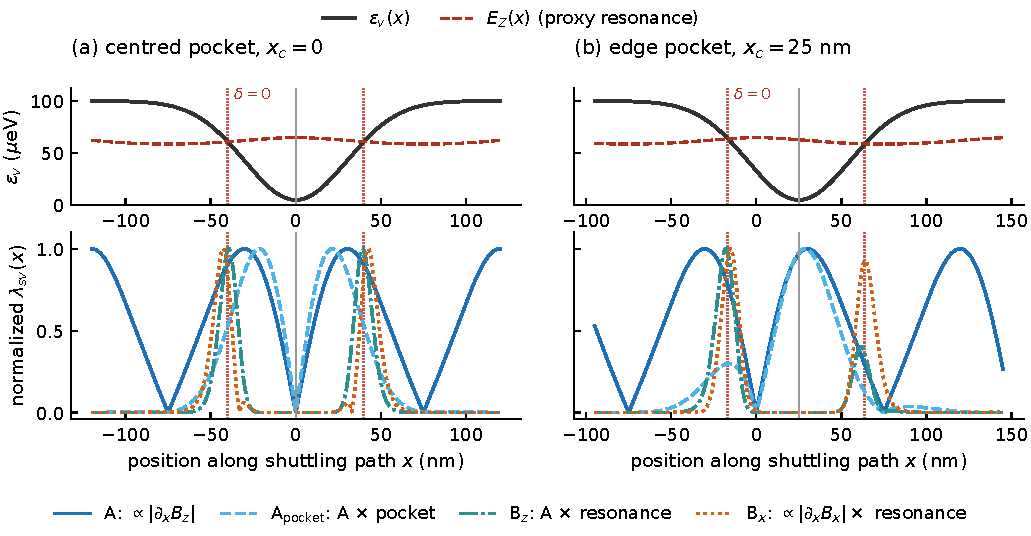
\includegraphics[width=\textwidth]{figures/coupling_profiles.pdf}
\caption{Valley detuning and the four coupling ans\"atze, for the two pocket
placements of the condition grid. Top row: the diabatic detuning
$\varepsilon_v(x)$ of Eq.~\eqref{eq:evx} against the local Zeeman energy
$E_Z(x)$ of Eq.~\eqref{eq:ez}. The red dotted verticals mark the two proxy
crossings, the positions where $\delta(x)\equiv\varepsilon_v(x)-E_Z(x)$
changes sign. They are not the pocket extent, which is set by $\sigma_p$; the
grey vertical marks the pocket centre. Bottom row: the four profiles, each
normalized to unit peak for shape comparison; the adopted prefactor convention
retains their unequal amplitudes in the simulations. (a)~Centred pocket. The
node of $|\partial_x B_z|$ at the array-symmetry point coincides with the
pocket bottom by placement, so A$_{\rm pocket}$ vanishes there despite its
pocket-centred envelope, and all three localized profiles form symmetric twin
peaks. (b)~Edge pocket, $x_c=25$~nm. The panel spans $x_c\pm4\sigma_p$, so
$\varepsilon_v$ is centred in it, but $E_Z(x)$ is periodic in the array and is
not symmetric about $x_c$, so the two crossings become inequivalent.
A$_{\rm pocket}$ is then single-flank dominated, and the two
resonance-localized profiles weight the crossings differently: because
$\partial_x B_z$ and $\partial_x B_x$ are approximately phase shifted, B$_z$ is
concentrated on the crossing at which $|\partial_x B_z|$ is larger, whereas
B$_x$ retains comparable weight at both. The crossing inequivalence is
induced by the off-centred placement, while its expression depends on the
gradient kernel.}
\label{fig:profiles}
\end{figure*}

$\Delta_v$ and $\sigma_E$ are phenomenological parameters rather than measured
constants. The geometric and velocity baselines are representative of reported
Si/SiGe shuttling devices.

We track valley excitation and valley-induced spin
dephasing~\cite{losert_strategies_2024,de_smet_high-fidelity_2025,volmer_mapping_2024,oda_suppressing_2026}
through two baseline-relative responses: the change in valley-leakage
probability $\Delta P_v$ and the change in dephasing phase variance
$\Delta\chi_\phi$ induced by the spin--valley coupling. The electron starts on
the \emph{lower} diabatic valley branch, and $P_v$ is the upper-branch
population at the end of the trajectory. The spin is initialized in
$\lvert+\rangle_s$, giving the four-level initial state
$\lvert+\rangle_s\otimes\lvert0\rangle_v$. We evaluate $P_v$ in the fixed
diabatic basis. At the trajectory endpoints $|\varepsilon_v|\gg\Delta_v$, so
this basis is nearly aligned with the instantaneous valley eigenbasis, although
the two do not coincide exactly for nonzero $\Delta_v$.

The two responses isolate different cross-effects and therefore use different
references. We compare a spin-only model with charge noise but no valley sector
($\mathrm{M1}$), a valley-aware reference without charge noise
($\mathrm{M1V}$), and the full model with charge noise and valley coupling
($\mathrm{M2}$):
$\Delta P_v=P_v^{\mathrm{M2}}-P_v^{\mathrm{M1V}}$ measures the effect of charge
noise on valley leakage, whereas
$\Delta\chi_\phi=\chi_\phi^{\mathrm{M2}}-\chi_\phi^{\mathrm{M1}}$ measures the effect of
the valley sector on charge-noise dephasing. The latter is computed within a
filter-function description of $1/f$ charge
noise~\cite{burkard_semiconductor_2023,struck_low-frequency_2020,viola_dynamical_1999}.
Thus $\mathcal{R}=(\Delta P_v,\Delta\chi_\phi)$ is a pair of cross-effect
diagnostics, not a decomposition of a single infidelity. Absolute performance
would instead be read from $P_v^{\mathrm{M2}}$ and
$\chi_\phi^{\mathrm{M2}}$ (or a derived phase-error proxy
$p_\phi=(1-e^{-\chi_\phi/2})/2$), which we do not optimize here.

Assuming that larger leakage and larger dephasing both reduce fidelity, we
classify each condition by the sign of each response that clears its
effect-size floor. The floors are $|\Delta P_v|\ge10^{-4}$ and
$|\Delta\chi_\phi|\ge10^{-3}$. A condition clearing both is \emph{robust} if
both responses improve, \emph{valley-trade} or \emph{spin-trade} if their signs
oppose, and \emph{both-worsen} if both worsen. If only one channel clears its
floor, the condition receives a separate single-channel category; if neither
does, it is below threshold. The floors are operational response-scale
criteria, not significance cutoffs, confidence bounds or external fidelity
standards. Their decade offset follows the decade separating the natural scales
of the two responses. Sensitivity to shared below-threshold assignments is
reported in the Supplementary Material, and classification stability is tested
by the seed-stable candidate screen of Sec.~\ref{sec:results}.

The realization count $n_{\rm real}$ denotes Monte-Carlo repetitions of the
simulated noise, not experimental repetitions, and matches the released data
tables and scripts. For a co-design decision, the direction of each channel
response---whether valley excitation and dephasing improve or worsen relative
to their channel-matched references---is itself relevant, not only the response
magnitude. We therefore use the thresholded sign pattern as the decision-facing
classification. The classification never compares the numerical magnitudes of
the two channels; each is judged against its own floor. The complementary
ranking diagnostic instead uses
$|\mathcal{R}|=\sqrt{\Delta P_v^2+\Delta\chi_\phi^2}$. Its ordering is
invariant to uniform rescaling but depends on the relative weighting of the two
channels, which we test explicitly below. The thresholded classification and
the magnitude ranking therefore answer different design questions.

\section{Methods}
\label{sec:methods}
\subsection{Condition grid and reference geometry}

We use two pocket placements: a centred case, $x_c=0$, aligned with the
array-symmetry point, and an off-centred edge case, $x_c=25$\,nm. For each
placement we scan nine geometries: the baseline plus one additive $+$ and $-$
step in each of four parameters, \texttt{period} ($\pm30$\,nm),
\texttt{depth} ($\pm10$\,nm), \texttt{half\_x} ($\pm5$\,nm) and
\texttt{half\_z} ($\pm3$\,nm). Here \texttt{depth} is the signed vertical
coordinate of the quantum well relative to the magnet plane, $-50$\,nm at
baseline; a $+$ step moves the well toward the magnet array and strengthens the
stray field. Combining the two placements, nine geometries, three velocities
and two coupling strengths ($\lambda=0.5$ and $1.0\,\mu$eV) gives 108
conditions and 432 ansatz--condition cells.

Each condition yields $\mathcal{R}=(\Delta P_v,\Delta\chi_\phi)$ of
Sec.~\ref{sec:model} and a nine-category label: four two-channel quadrants (\emph{robust},
\emph{valley-trade}, \emph{spin-trade}, \emph{both-worsen}), four
single-channel categories and \emph{below-threshold}. We reserve
``quadrant'' for the four two-channel labels and use
\emph{classification agreement} for exact agreement of the nine-category
label. Because the label is a bijection of the two channels' three-state
descriptions (improve, inactive, worsen), it also supports the channel-resolved
diagnostics below. The effect-size floors are operational criteria rather than
significance cutoffs or Monte-Carlo confidence bounds.

\subsection{Matched cross-ansatz and cross-seed comparison}

The primary comparison asks how much the design-facing label changes with the
coupling profile relative to a change of random sample alone. We evaluate the
full grid in five seed blocks. Within each block all four ans\"atze use common
random numbers, so cross-ansatz comparisons share one realization set; the
blocks themselves use disjoint seeds. Each block is evaluated at nested
$n_{\rm real}=5,10,20,30,40,60,80,100$, with smaller counts forming prefixes of
the larger counts.

Let $L_{acb}$ denote the nine-category label of condition
$c\in\mathcal{C}$ under ansatz $a\in\mathcal{A}$ in block
$b\in\mathcal{B}$, with $|\mathcal{C}|=108$, $|\mathcal{A}|=4$ and
$|\mathcal{B}|=5$. For each ansatz pair and block pair,
%
\begin{align}
d_{aa'} &= \big\langle \mathbf{1}[L_{acb}\neq L_{a'cb}] \big\rangle_{c,b},
\nonumber\\
d_{bb'} &= \big\langle \mathbf{1}[L_{acb}\neq L_{acb'}] \big\rangle_{c,a},
\label{eq:pairwise-d}
\end{align}
%
where each average runs over the cells in which both pair members exist. We
then average uniformly over the six ansatz pairs and ten block pairs,
%
\begin{equation}
D_{\rm ansatz} = \frac{1}{6}\!\!\sum_{a<a'}\! d_{aa'},
\qquad
D_{\rm seed} = \frac{1}{10}\!\!\sum_{b<b'}\! d_{bb'} .
\label{eq:D}
\end{equation}
%
We also report all sixteen pairwise values,
$\Delta_D=D_{\rm ansatz}-D_{\rm seed}$ and
$R_D=D_{\rm ansatz}/D_{\rm seed}$. Complete separation of the two pairwise
distributions would imply uniform dominance, but no numerical separation
threshold is imposed.

These estimands are comparative summaries, not additive uncertainty
components. $D_{\rm ansatz}$ is evaluated from finite samples and therefore
retains an ansatz$\times$realization interaction. $D_{\rm seed}$ measures
finite-sampling instability of the thresholded label rather than estimator
variance. In particular, $D_{\rm ansatz}+D_{\rm seed}$ has no decomposition
interpretation.

A shared \emph{below-threshold} assignment counts as agreement. We therefore
report $p_{\rm all}$, the fraction of conditions inactive under every ansatz and
block; $B_{\rm ansatz}$ and $B_{\rm seed}$, the fractions of pairwise
comparisons in which both members are below threshold; and their share of total
agreement, $B/(1-D)$. As a sensitivity analysis, we also recompute
disagreement on the union of comparisons in which at least one pair member has
a two-channel quadrant label. We do not use intersection conditioning.

\subsection{Channel-resolved diagnostics}

The two responses are isolated against different references by construction, so
they carry different baselines and are never pooled. We therefore repeat the
comparison on each channel's three-state description, which satisfies the
exact identity
\begin{equation}
D_{\rm joint} = D_{P} + D_{\chi} - D_{\rm both}
\label{eq:channel-identity}
\end{equation}
for both the ansatz and the seed averages, $D_{\rm both}$ being the fraction of
comparisons that differ in both channels. Equation~\eqref{eq:channel-identity} is an
inclusion--exclusion relation: the joint estimand combines the two channel
disagreements and their overlap. A near-equality of $D_{\rm ansatz}$ and
$D_{\rm seed}$ can therefore arise from opposing channel-level contrasts
together with the overlap term. The three contributions must therefore be
interpreted jointly.

For the continuous responses we use a per-channel pairwise dispersion
$S^{(q)}$, structurally parallel to the label estimand. Writing $R^{(q)}_{acb}$
for channel $q$ of the response and $f_q$ for that channel's floor,
%
\begin{equation}
S^{(q)}_{\rm ansatz} =
\Big\langle \big[(R^{(q)}_{acb}-R^{(q)}_{a'cb})/f_q\big]^2
\Big\rangle^{1/2}_{a<a',\,c,\,b},
\label{eq:S}
\end{equation}
%
and $S^{(q)}_{\rm seed}$ likewise over block pairs at fixed ansatz. For any finite set of $m$ values,
$\sum_{i<j}(x_i-x_j)^2 = m\sum_i(x_i-\bar{x})^2$. The mean pairwise squared
difference is therefore exactly twice the sample variance with the $(m-1)$
divisor. The $4$-versus-$5$ group-size asymmetry consequently cancels.
$S^{(q)}$ is therefore exactly $\sqrt{2}$ times a sample standard deviation---an
algebraic identity, not a distributional assumption. $S^{(q)}$ is a dispersion of pairwise differences and carries no
information about whether the underlying responses clear their floors.

\subsection{Candidate selection and transport}

Operating-point candidates are selected from seed stability at the
(ansatz, condition) level. A pair is a candidate when the condition is labelled
robust under that ansatz in all three discovery blocks; cross-ansatz agreement
does not enter selection. Blocks 1--3 form the discovery set and blocks 4--5
the holdout. Every condition in the discovery union $U^{\rm disc}$ is then
evaluated on the holdout blocks under all four ans\"atze, yielding a
within-ansatz replication count and a transport count from 0 to 4. Because
$U^{\rm disc}$ changes with ensemble size, transport is reported as counts
rather than a rate. Repeating the screen at $n_{\rm real}=100$ gives an
\emph{extended confirmation}, not an independent second holdout: the larger
aggregate contains the $n_{\rm real}=30$ realizations as a prefix and reuses
the same holdout blocks.

\subsection{Registration and the ranking diagnostic}

The estimands, candidate-selection rule and checkpoints
$n_{\rm real}=5,10,20,30$, with primary endpoint $n_{\rm real}=30$, were fixed
in writing before data generation. The extension to $n_{\rm real}=100$ was registered
after the $n_{\rm real}=30$ result and before generation of the extension
data, including its checkpoints, hard stop and reporting language. The channel
decomposition of Eq.~\eqref{eq:channel-identity}, the family breakdowns and the
ranking diagnostic below were introduced after inspection of the results and
are identified as post-hoc.

For the ranking diagnostic we compute the pairwise Spearman correlation of
$|\mathcal{R}|$ across conditions within each seed block and average over
blocks. Because the released magnitude is unnormalized whereas the classifier
judges each channel against its own floor, we also recompute the ranking under
floor-normalized and single-channel magnitudes and under signed
$\Delta\chi_\phi$.

The analysis makes no population-level statistical claim. There are five
registered seed blocks, and grid cells paired by common random numbers across
geometry, case and ansatz are not independent replicates. We therefore do not
resample them as i.i.d., report confidence intervals, or perform significance
tests; threshold-dependent statements remain conditional on the operational
floors.

Figure~\ref{fig:quadrant} illustrates why ranking and classification are kept
separate. Two ans\"atze can order conditions by response magnitude almost
identically while assigning many of them to different thresholded categories.
The ranking summarizes response magnitude, whereas the label records which
response signs are resolved above their channel-specific floors. A final
performance decision would additionally require the absolute full-model leakage
and dephasing proxies, which are outside the optimization performed here.

\begin{figure*}[!tp]
\centering
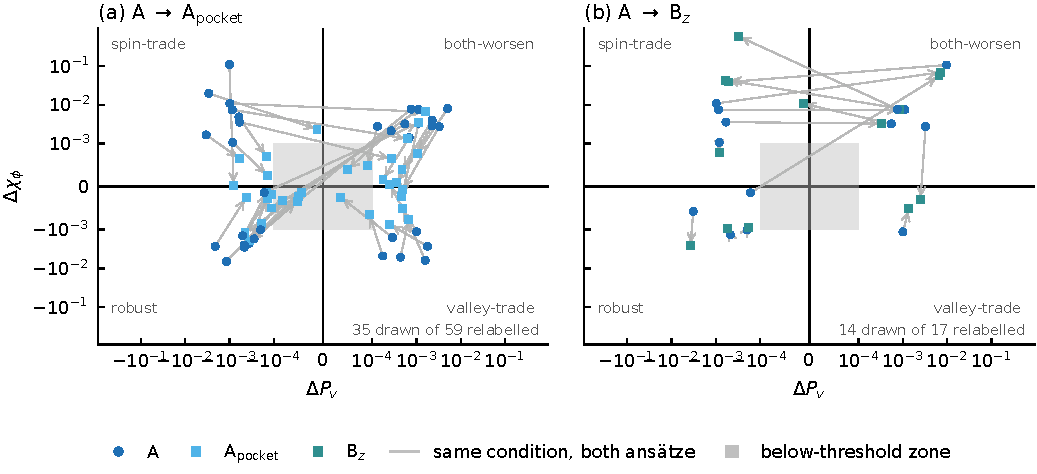
\includegraphics[width=\textwidth]{figures/quadrant_data.pdf}
\caption{Where the design-facing classification changes between ans\"atze, at
$n_{\rm real}=100$ in one seed block. Each arrow joins the response
$\mathcal{R}=(\Delta P_v,\Delta\chi_\phi)$ of one condition under the first
ansatz to its response under the second. Only relabelled conditions are drawn,
and of those only comparisons in which at least one member carries a
two-channel quadrant label, the union restriction of Sec.~\ref{sec:methods};
both counts are given on each panel. The grey box is the below-threshold zone
set by the operational floors $|\Delta P_v|\ge10^{-4}$ and
$|\Delta\chi_\phi|\ge10^{-3}$, and the axes are symmetric-log with the linear
core set to those floors, so the box is the linear region. (a)~A against
A$_{\rm pocket}$, the pair with the lowest classification agreement in the
family, $0.467$. (b)~A against B$_z$, the highest, $0.839$. Their rank
correlations differ by only $0.011$, $0.967$ against $0.978$, so the two panels
show nearly identical magnitude ordering despite markedly different labels. One
seed block is shown for visual clarity; the reported agreement values average
over all blocks.}
\label{fig:quadrant}
\end{figure*}

\paragraph*{AI-assisted review.}
Large-language-model tools were used as secondary review aids during
post-processing and manuscript preparation: ChatGPT (OpenAI; GPT-5.5 and
GPT-5.6 Sol) and Claude (Anthropic; Opus 4.8 and Opus 5). They reviewed
scientific reasoning and claim scope, inspected and debugged simulation,
analysis, plotting and verification code, and checked consistency among the registered
estimands, the archived analysis outputs, the figures and the manuscript text.
The purpose was to reduce implementation and transcription errors and to add a
second consistency check. The registered Monte-Carlo runs were executed by the
author. Every suggested code or text change was reviewed by the author, and
every reported numerical value was verified against the archived outputs. The
final interpretations and conclusions were determined by the author.

\section{Results}
\label{sec:results}

\begin{figure*}[!tp]
\centering
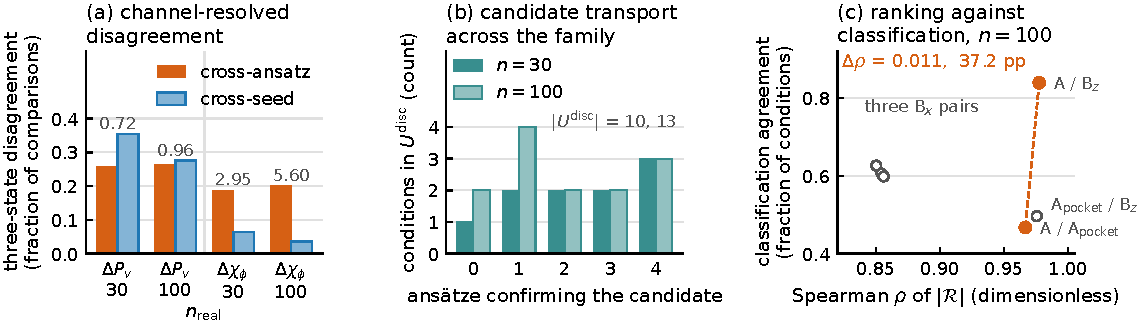
\includegraphics[width=\textwidth]{figures/sensitivity_atlas.pdf}
\caption{Channel structure, candidate transport, and the ranking
diagnostic. (a)~Three-state disagreement per response channel,
cross-ansatz against cross-seed, at both endpoints; the number above each
pair is their ratio. The valley channel moves from sampling-led at
$n_{\rm real}=30$ to approximately balanced at $100$, while the dephasing
channel's cross-ansatz excess grows. Post-hoc diagnostic. (b)~Conditions in
the discovery union $U^{\rm disc}$, binned by how many of the four ans\"atze
confirm them on the holdout blocks; the two columns are $n_{\rm real}=30$
(pre-registered) and $100$. $|U^{\rm disc}|$ is 10 at $n_{\rm real}=30$
and 13 at $100$. The $n_{\rm real}=100$ column is an extended confirmation on
the same holdout blocks, so the counts are not a before-and-after on one
cohort. (c)~Pairwise Spearman rank correlation of
$|\mathcal{R}|$ against classification agreement, six ansatz pairs at
$n_{\rm real}=100$. Filled markers joined by the dashed line are the
counterexample pair, open markers the other four. A/A$_{\rm pocket}$ and
A/B$_z$ differ by
$0.011$ in rank correlation and $0.372$ in classification
agreement. The three pairs containing B$_x$ group together in the middle band.
Post-hoc diagnostic.}
\label{fig:atlas}
\end{figure*}

\paragraph{Unmatched seeds exaggerated the archived model disagreement.}
The archived analysis used a separate noise realization for each ansatz, so
its cross-ansatz comparison also contained a sampling difference. Repeating the
comparison at $n_{\rm real}=5$ with matched seed block and the same archived
observable convention raises mean classification agreement from $35.96\%$ to
$56.94\%$ and mean rank correlation from $0.837$ to $0.917$. The disagreement falls from $64.04\%$ to $43.06\%$, a reduction
of about one third. These values are retained only as an
archived seeding audit and are not mixed with the corrected T0-C results.

\paragraph{Matched cross-ansatz disagreement remains substantial.}
At the pre-registered endpoint $n_{\rm real}=30$,
$D_{\rm ansatz}=0.388$ and $D_{\rm seed}=0.385$. Thus roughly $39\%$ of matched
comparisons change their design-facing label across ans\"atze, while a change
of seed block produces a comparable rate.

The aggregate contains a stable pairwise structure. Across all eight registered
checkpoints, A/B$_z$ forms the lowest-disagreement tier
($0.143$--$0.180$); the three pairs containing B$_x$ form a narrow middle band
($0.348$--$0.407$); and A/A$_{\rm pocket}$ together with
A$_{\rm pocket}$/B$_z$ form the highest tier ($0.467$--$0.533$).
A$_{\rm pocket}$/B$_x$ lies in the middle band. From
$n_{\rm real}=30$ to $100$ no ansatz pair moves by more than $0.020$,
whereas the seed-pair mean falls from $0.385$ to $0.298$. These tiers describe the six specified pairwise contrasts within the
four-profile family; they do not rank underlying physical modeling axes. Even
the most similar pair,
A/B$_z$, disagrees on $0.161$ of conditions at $n_{\rm real}=100$.

The ansatz- and seed-pair distributions nevertheless overlap at every
checkpoint, so uniform dominance does not hold. At $n_{\rm real}=100$ the
lowest seed-pair disagreement is $0.169$ and the lowest ansatz-pair value is
$0.161$; the remaining ranges interleave. In a post-hoc count over the same
sixty pairwise comparisons, 46 favour the ansatz side at $n_{\rm real}=100$,
compared with 33 at $n_{\rm real}=30$. Shared inactivity contributes to both
forms of agreement: 13 of 108 conditions are below threshold under every
ansatz and block at $n_{\rm real}=100$, and shared below-threshold assignments
account for $0.464$ of ansatz-pair agreement. Restricting the comparison to the
union in which at least one pair member has a two-channel quadrant label
increases the contrast to $0.521$ versus $0.323$.

\paragraph{Sampling and ansatz disagreement scale differently with ensemble size.}
Across the eight checkpoints, $D_{\rm seed}$ decreases from $0.542$ to
$0.298$ without a rebound, whereas $D_{\rm ansatz}$ remains between $0.369$ and
$0.395$ [Fig.~\ref{fig:overview}(d)]. The ordering reverses between
$n_{\rm real}=20$ and $30$ and the separation grows thereafter, with $R_D$
rising from $0.73$ to $1.33$. Cross-seed disagreement is therefore strongly
ensemble-size dependent over the registered trajectory, whereas cross-ansatz
disagreement persists across the ensemble sizes and registered seed blocks
examined.

This trajectory does not establish an asymptotic limit. $D_{\rm seed}$ is still
decreasing at the $n_{\rm real}=100$ hard stop, and $D_{\rm ansatz}$ retains a
finite-sample ansatz$\times$realization interaction. Its observed flatness is
therefore an empirical property of this design and ensemble range, not a
property of the model family. Up to the primary
$n_{\rm real}=30$ endpoint the two disagreement scales are comparable, which
makes the same-size cross-seed benchmark essential for interpreting
cross-ansatz disagreement.

\paragraph{The balance depends on the response channel.}
Because the nine-category label is a bijection of the two channels'
three-state descriptions, Eq.~\eqref{eq:channel-identity} decomposes joint
disagreement by inclusion--exclusion [Fig.~\ref{fig:atlas}(a)]. At the primary
endpoint, the valley and dephasing contrasts have opposite signs, and the
overlap term leaves the joint difference near zero. Specifically, at
$n_{\rm real}=30$, valley disagreement is larger across seeds than across
ans\"atze ($0.355$ versus $0.257$), whereas dephasing shows the opposite
ordering ($0.188$ versus $0.064$). The channel contrasts, $-0.099$ and
$+0.124$, together with the overlap term $-0.023$ leave the joint difference
near zero, $+0.002$. At $n_{\rm real}=100$ the valley channel is approximately
balanced, with a cross-ansatz to cross-seed ratio of $0.96$, while the
dephasing ratio reaches $5.60$.

The continuous diagnostics sharpen this channel contrast: dephasing
cross-ansatz dispersion changes little between the two endpoints while its
cross-seed dispersion falls, whereas both valley dispersions decrease. For
$\Delta\chi_\phi$, cross-ansatz dispersion stays between $40$ and $52$ floor
units over the trajectory and changes from $43.5$ to $42.4$ between the two
endpoints, while cross-seed dispersion falls from $21.8$ to $9.8$. For
$\Delta P_v$, both dispersions decrease substantially: cross-ansatz from
$28.8$ to $23.0$ and cross-seed from $36.2$ to $19.0$, giving a final ratio of
only $1.22$. Neither continuous dispersion is monotone in $n_{\rm real}$;
the cross-seed dispersion rebounds at $n_{\rm real}=60$ for $\Delta P_v$ and
at $n_{\rm real}=10$ for $\Delta\chi_\phi$. $D_{\rm seed}$ is the only
quantity here that decreases monotonically across all eight registered
checkpoints. Which response a design criterion emphasizes therefore
changes the relative size of model-form and sampling sensitivity.

\paragraph{Ranking agreement does not predict classification agreement.}
The ranking diagnostic and all comparisons in this paragraph are post-hoc. At
$n_{\rm real}=100$, pairwise rank correlation is high across the family
(mean $0.913$, range $0.850$--$0.978$), while classification agreement is
much broader (mean $0.605$, range $0.467$--$0.839$). The two summaries do not track one another
[Fig.~\ref{fig:atlas}(c)]: A/A$_{\rm pocket}$ and A/B$_z$ differ by only
$0.011$ in rank correlation but by $0.372$ in classification
agreement. Cohen's $\kappa$ spans $0.311$--$0.804$, so chance correction does
not remove the disparity.

To test whether the decoupling is an artifact of channel weighting, we
recomputed the ranking under floor-normalized and single-channel magnitudes.
The A/A$_{\rm pocket}$--A/B$_z$ rank-correlation gap increases only from
$0.011$ to $0.023$ under floor normalization, and the single-channel
magnitudes change it less.

Among the ranked quantities examined, signed
$\Delta\chi_\phi$ separates the pair most strongly: its gap is $0.147$, versus
$0.042$ for signed $\Delta P_v$ and $0.011$ for the released magnitude. Across
the six ansatz pairs, its Spearman correlation with classification agreement is
$+0.486$ at both $n_{\rm real}=30$ and $100$, compared with $-0.086$ for the
released magnitude. This suggests that spin-response sign contributes to the
decoupling, but the evidence is descriptive: the metric is post-hoc, the six
pairs are not independent, and the classifier also depends on floor crossing.

\begin{table*}[!tbp]
\centering
\caption{Seed-stable candidates at the pre-registered endpoint
$n_{\rm real}=30$. Selection uses the three discovery blocks and seed stability
alone, under a single ansatz; cross-ansatz agreement is never a selection
criterion. ``discovered by'' lists the ans\"atze under which the condition is
robust in all three discovery blocks, and ``confirmed'' counts the ans\"atze
under which it is robust in both holdout blocks. Geometry labels denote the
signed step from the baseline point.}
\label{tab:retest}
\small
\begin{tabular}{llccll}
\toprule
case & geometry & $v$\,(m/s) & $\lambda$\,($\mu$eV) & discovered by & confirmed \\
\midrule
center & \texttt{period}$-$   & 5  & 1.0 & A$_{\rm pocket}$                 & 2/4 \\
edge   & \texttt{depth}$-$    & 5  & 1.0 & A, A$_{\rm pocket}$, B$_z$, B$_x$& \textbf{4/4} \\
edge   & \texttt{half\_z}$-$  & 5  & 1.0 & A                           & 2/4 \\
edge   & \texttt{period}$+$   & 5  & 1.0 & A, A$_{\rm pocket}$, B$_x$       & \textbf{4/4} \\
edge   & \texttt{depth}$+$    & 10 & 0.5 & A, B$_z$, B$_x$             & 3/4 \\
edge   & \texttt{depth}$+$    & 10 & 1.0 & A, A$_{\rm pocket}$, B$_z$, B$_x$& \textbf{4/4} \\
edge   & \texttt{baseline}    & 20 & 1.0 & B$_z$, B$_x$                & 1/4 \\
edge   & \texttt{half\_z}$+$  & 20 & 1.0 & A, B$_z$, B$_x$             & 3/4 \\
edge   & \texttt{half\_z}$-$  & 20 & 1.0 & B$_x$                       & 1/4 \\
edge   & \texttt{period}$+$   & 20 & 1.0 & A, B$_z$, B$_x$             & 0/4 \\
\bottomrule
\end{tabular}
\end{table*}

\paragraph{Seed-stable candidates transport unevenly.}
Selection on seed stability across the three discovery blocks yields 25
(ansatz, condition) candidate pairs at $n_{\rm real}=30$, distributed 7/4/6/8
over A, A$_{\rm pocket}$, B$_z$ and B$_x$, with a union of ten conditions
(Table~\ref{tab:retest}). On the two holdout blocks, 21 of the 25 pairs
replicate within their original ansatz.

Transport across ans\"atze is less uniform [Fig.~\ref{fig:atlas}(b)]. Of the ten
conditions, one is confirmed under no ansatz, two under one, two under two, two
under three and three under all four. The registered $n_{\rm real}=100$
companion analysis is an extended confirmation: it contains 31 pairs and a
union of 13 conditions, with 21 of 31 replicating within ansatz. The numbers of
conditions confirmed under zero, one, two, three, and four ans\"atze are 2, 4,
2, 2, and 3, respectively. Because the larger
aggregate contains the $n_{\rm real}=30$ realizations as a prefix and reuses
the same holdout blocks, it is not an independent replication. Of the original
25 pairs, 22 are retained, 3 are lost and 9 are gained; the same three
conditions receive four-of-four confirmation at both prefixes. These are
grid-local candidates within the diagnostic family, not evidence for a general
ranking of robust geometries.


\section{Discussion}

The matched comparison shows that design-facing classifications in this setting
depend substantially on the assumed coupling profile. The nine-category label
changes even when the geometry, operator structure, noise model and random
realizations are held fixed. This dependence is visible in the candidate layer
as well: among the ten seed-stable conditions at $n_{\rm real}=30$, three are
confirmed under all four ans\"atze and one under none.

The cross-seed benchmark changes how that dependence should be interpreted.
Cross-ansatz disagreement remains near $0.39$ over a twentyfold increase in
ensemble size, while cross-seed disagreement falls from $0.542$ to $0.298$.
At the smaller registered checkpoints the two scales are comparable, so
cross-ansatz disagreement cannot be interpreted without specifying the
finite-sampling scale at the same $n_{\rm real}$. The archived seeding audit
makes the same point from another direction: matching realizations removes
about one third of its apparent disagreement, while most of the difference
between profiles remains.

Aggregate disagreement does not determine whether rankings and classifications
agree. High rank correlation does not guarantee classification agreement.
A/A$_{\rm pocket}$ provides the clearest example: its response-magnitude
ranking is close to that of A/B$_z$, yet its classification agreement is the
lowest in the family.

The channel balance is likewise uneven. Dephasing shows a large cross-ansatz
excess at both endpoints, whereas valley excitation has larger cross-seed
disagreement at $n_{\rm real}=30$ and is approximately balanced at $100$. The
six ansatz pairs also separate into three persistent disagreement tiers across
all eight registered checkpoints. These tiers characterize the specified
contrasts in this family; they do not identify a general causal axis of model
uncertainty.

This model-form sensitivity matters because no generally validated effective
local spin--valley kernel is yet available for the shuttled-dot/micromagnet
regime. A microscopically derived kernel would provide a preferred physical
description and could reduce the profile ambiguity studied here. The same comparison would
remain useful for residual parameter or structural uncertainty. Valley
landscapes constrained by alloy-disorder calculations and conveyor-mode
measurements~\cite{paquelet_wuetz_atomic_2022,losert_practical_2023,volmer_mapping_2024}
can be incorporated directly when they map onto the same effective operator
structure. A microscopic derivation that changes the operator structure would
instead extend the comparison to operator-form uncertainty.

\paragraph{Corrective replication.}
A later implementation audit corrected the valley-energy ordering, after which
the $n_{\rm real}=30$ and $n_{\rm real}=100$ production runs were repeated.
The registered estimands, effect-size floors, seed design, candidate rule,
checkpoints and $n_{\rm real}=100$ hard stop were unchanged. All current values
reported here come from those repeated runs.

\paragraph{Limitations.}
The conclusions are conditional on four diagnostic scalar coupling profiles,
one fixed minimal spin--valley operator, one charge-noise description and the
periodic micromagnet reference geometry. Operator-level alternatives are not
sampled. The same $1/f$ spectrum and one representative,
non-device-calibrated displacement-noise amplitude enter both responses, so the
study isolates coupling-profile dependence against that fixed noise model
rather than scanning noise-spectrum or amplitude uncertainty.

The thresholded labels are operational classifications under the stated
effect-size floors, not confidence-certified assignments. Sensitivity to shared
below-threshold assignments is reported in the Supplementary Material. A
post-hoc independent factor-of-two sweep of both operational floors leaves the
$n_{\rm real}=100$ cross-ansatz versus cross-seed ordering and the pairwise
disagreement-tier structure unchanged, while the exact crossover checkpoint is
floor dependent (Supplementary Material). The five seed blocks and the
common-random-number grid do not constitute
independent population replicates, and we report no confidence intervals or
significance tests.

The registered trajectory ends at $n_{\rm real}=100$ while cross-seed
disagreement is still decreasing, so no convergence or asymptotic claim is
made. Cross-ansatz disagreement also retains a finite-sample
ansatz$\times$realization interaction. The $n_{\rm real}=100$ candidate layer is
an extended confirmation using the same block structure and a nested
realization prefix, not an independent replication. The three conditions
confirmed under all four ans\"atze are therefore grid-local results within this
diagnostic family.

These restrictions deliberately hold the geometric backdrop fixed so that
coupling-profile dependence can be isolated.

\paragraph{Implications for co-design.}
A robust operating-point claim should identify the coupling profile under which
it was obtained and test whether the point transports across a justified
family. The same applies to proposed mitigations based on shuttling velocity,
dot shape or path~\cite{losert_strategies_2024}. Cross-ansatz comparisons should
also carry a same-ansatz cross-seed benchmark at the same ensemble size,
because the two scales are comparable at the smaller checkpoints studied here.

The atlas supplies that cross-profile test within the four diagnostic profiles
studied here, for both the classification and the seed-stable candidates. It
does not supply the independent constraint on the coupling that would remove
the ambiguity.

\section{Conclusion}

Using matched random realizations, we compared the sensitivity of a
design-facing classification to the coupling ansatz with its sensitivity to
finite Monte-Carlo sampling. In the archived analysis, separate realization sets inflated cross-ansatz
disagreement; matching removes about one third of that archived disagreement. In the corrected paired comparison,
cross-seed disagreement decreases strongly with ensemble size while
cross-ansatz disagreement remains substantial over the registered range.

The imbalance is response dependent. Dephasing is much more sensitive to the
ansatz than to the seed block at $n_{\rm real}=100$, whereas valley excitation
is approximately balanced. Magnitude ranking and thresholded classification
also capture different aspects of the response, and seed-stable candidates
transport unevenly across the four profiles. For this diagnostic family, a
design conclusion obtained from one phenomenological coupling therefore
remains model-conditional unless the coupling is independently constrained or
the conclusion is shown to persist across a justified family.

\paragraph{Future work.}
A microscopic effective $H_{sv}$ for the shuttled-dot/micromagnet regime could
be derived from orbital admixture, valley--orbit interaction and $g$-factor
anisotropy~\cite{friesen_theory_2010,hosseinkhani_theory_2022,zhang_controlling_2021}.
Related work on gradient, strain and spin--orbit design in Ge hole-spin
platforms~\cite{sarkar_effect_2025,mauro_strain_2025,geyer_anisotropic_2024,hendrickx_sweet-spot_2024,jin_probing_2024}
provides complementary examples of how those microscopic ingredients can enter
device-level design. A microscopic model with the same effective
operator structure can enter the present framework as an additional profile;
one with a different structure would extend the comparison to operator-form
uncertainty. A separate factorial design would be required to attribute the
observed disagreement to gradient component, spatial localization or other
physical axes.


\section*{Acknowledgments}
The author thanks the members of the Quantum Computing Research Group
(QCRG), Korea, for helpful discussions. This research received no specific
grant from any funding agency in the public, commercial, or not-for-profit
sectors.

\section*{Author declarations}
\subsection*{Conflict of interest}
The author has no conflicts to disclose.

\subsection*{Ethics approval}
This work is entirely theoretical and computational. It involved no human
participants, animal subjects, or personal data, and required no ethical
approval.

\subsection*{Author contributions}
\textbf{Inuk You:} Conceptualization (lead); Data curation (lead); Formal
analysis (lead); Investigation (lead); Methodology (lead); Software (lead);
Validation (lead); Visualization (lead); Writing -- original draft (lead);
Writing -- review \& editing (lead).

\section*{Data availability}
The data that support the findings of this study are openly available in
Zenodo at
\href{https://doi.org/10.5281/zenodo.21588784}{https://doi.org/10.5281/zenodo.21588784},
reference number~21588784~\cite{you_reproducibility_2026} (all versions:
\href{https://doi.org/10.5281/zenodo.21588003}{10.5281/zenodo.21588003}), and
are mirrored at \url{https://github.com/youinuk/spin-valley_model}. The
archive contains the simulation code, the analysis outputs behind every
reported number, and the scripts that regenerate every figure. All quantitative
results of the matched comparison are reproducible from those outputs with the
registered seed blocks; quantities identified in the text as archival retain
the seeding and release provenance of the earlier record.

\bibliographystyle{aipnum4-2}
\bibliography{ref}

\end{document}
